\section{PCB Design}

	\subsection{Definition High Speed Circuits}
		A circuit is high speed, if we need to consider the signal traces as transmission lines. \\
		\textbf{Rule of Thumb}:\\
		For a given signal having a rise/fall time $t_r$, a signal trace of length $l$ must be considered under the transmission line theory, if:
		\begin{equation}
			t_r < 2\tau 
		\end{equation}
		where $\tau$ is the time the signal takes to travel the distance $l$. 
		\begin{equation}
			\tau = \frac{l}{v_{ph}} 
		\end{equation}		
		where $v_{ph}$is the signal velocity (typ. values for PCB 0.5c ... 0.6c).\\
		Example: \\
		Having a rise time of 2 ns and a signal velocity of 0.5c, the transmission line effects occur at a length of: 
		\begin{equation}
			l = \tau v_{ph} > \frac{t_r}{2}v_{ph} = \frac{2\cdot 10^{-9}}{2}\cdot 1.5 \cdot 10^8 m/s = 15 cm
		\end{equation}	
	\subsection{PCB Partitioning and Shielding}
	Separate inside from outside world. Inside world contains the protected filtered area whereas the outside world contains any unshielded cable, connector, components and PCB traces that are not over a continuous reference plane, pins or heat sinks that are taller than $\lambda/10$.\\
	Goal: Reduce design iterations, costly shielding and fixes! \\
	\textbf{Dividing the inside world further: }
	\begin{itemize}
		\item Identify functional blocks having different signal properties (analog, noisy, RF I/O)
		\item Keep high speed clock sources far from connectors
		\item Separate noisy blocks (e.g. switching power supplies) from sensitive analog circuits
		\item Carefully rout signals leaving one zone for another 
		\item Apply adequate filtering or suppressing to these signals
		\item Be cautious when using Autorouter
	\end{itemize}
	\textbf{Self generated Problems:}
	\begin{itemize}
		\item Different internal blocks can affect each other with EM phenomena: 
			\begin{itemize}
				\setlength{\itemsep}{-5pt}
				\item Noise emitted by PWM circuits (power switching, motor drives, inverters)
				\item GND noise generated by fast switching logic circuits
				\item RF noise from oscillators or wireless transceivers
				\item Harmonics due to signal distortion, inter modulation
				\item Spurious signals generated by unwanted demodulation
			\end{itemize}
		\item Possible coupling of these phenomena
			\begin{itemize}
				\setlength{\itemsep}{-5pt}
				\item Through common power supply
				\item Capacitively, Inductively
			\end{itemize}
		\item Possible prevention of noise from crossing a functional block's boundary
			\begin{itemize}
				\setlength{\itemsep}{-5pt}
				\item Ferrite beads
				\item Filters
				\item Optocouplers
				\item Common mode chokes
				\item Fibre optic link instead of copper cable
				\item Add series impedance to I/O signals
				\item Adequately filter signals going to the front panel against ESD by using one of the above techniques
				\item Add shielding at PCB level before shielding at cabinet level (reduced weight, cost and often not possible due to wireless systems)
			\end{itemize}
	\end{itemize}
		\subsubsection{Waveguides}
		A waveguide allows an EM wave to propagate above a certain frequency $f_c$, above this frequency the attenuation is very low, below $f_c$ the attenuation is very strong. 
		\begin{figure}[h]
			\centering
			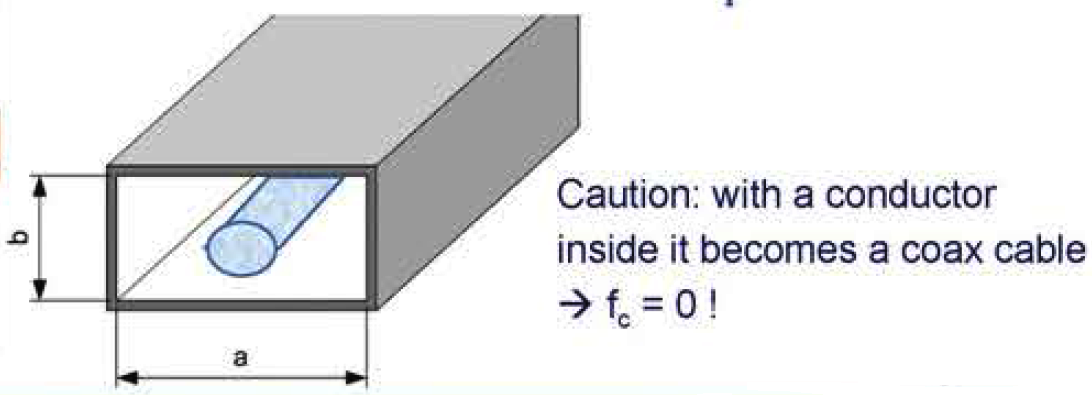
\includegraphics[width=0.5\textwidth]{images/Waveguide.png}
			\caption{Waveguide}
			\label{Fig:Waveguide}
		\end{figure}
		\begin{equation}
			f_c = \frac{\lambda_c}{2}
		\end{equation}
		with 
		\begin{equation}
			\lambda_c = \frac{c}{f_c}
		\end{equation}
		\textbf{Waveguides and PCB Design?} 
		\begin{itemize}
			\item Waveguide properties can be used to block signal propagation through the apertures inside the PCB, which is accomplished by overlaying guard rings (top layer) and reference planes (internal layer) over a distance of $\lambda/10$ or more in order to create waveguides of this depth. 
			\item Place as many blind vias on the waveguide's side walls as possible
			\item Keep aperture of the waveguides so that < $\lambda/2$ (at the highest signal frequency)
			\item Do not pass signal traces inside these waveguides
		\end{itemize}
		\begin{figure}[h]
			\centering
			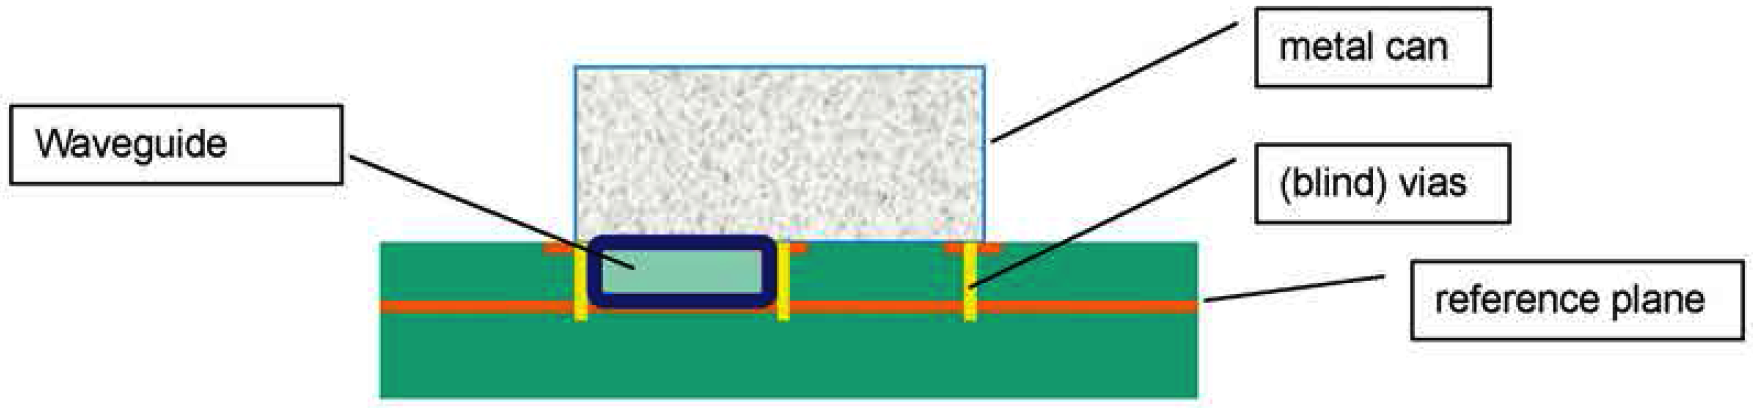
\includegraphics[width=0.75\textwidth]{images/PCBWaveguides.png}
			\caption{Waveguide on PCB}
			\label{Fig:PCBWaveguide}
		\end{figure}
		\textbf{Waveguide as Resonator} \\
		A closed metal box has many resonance frequencies inside. The lowest resonant frequency is ag $f_0 = \frac{c}{2a}$, where a is the broadest side length of the box. Resonances are often unwanted inside the metal can since they change the circuit's behaviour (increased coupling, HF currents etc) A metal can having resonances inside has a decreases shielding effect.\\
		Therefore: 
		\begin{itemize}
			\item Keep metal cans as small as possible
			\item Make small compartments inside
			\item If necessary, coat the inner of the metal can with a film of absorbing material (ferrite)
		\end{itemize} 
		\subsubsection{Vias: blind (buried) vs. pass-through}
			\begin{figure}[h!]
				\centering
				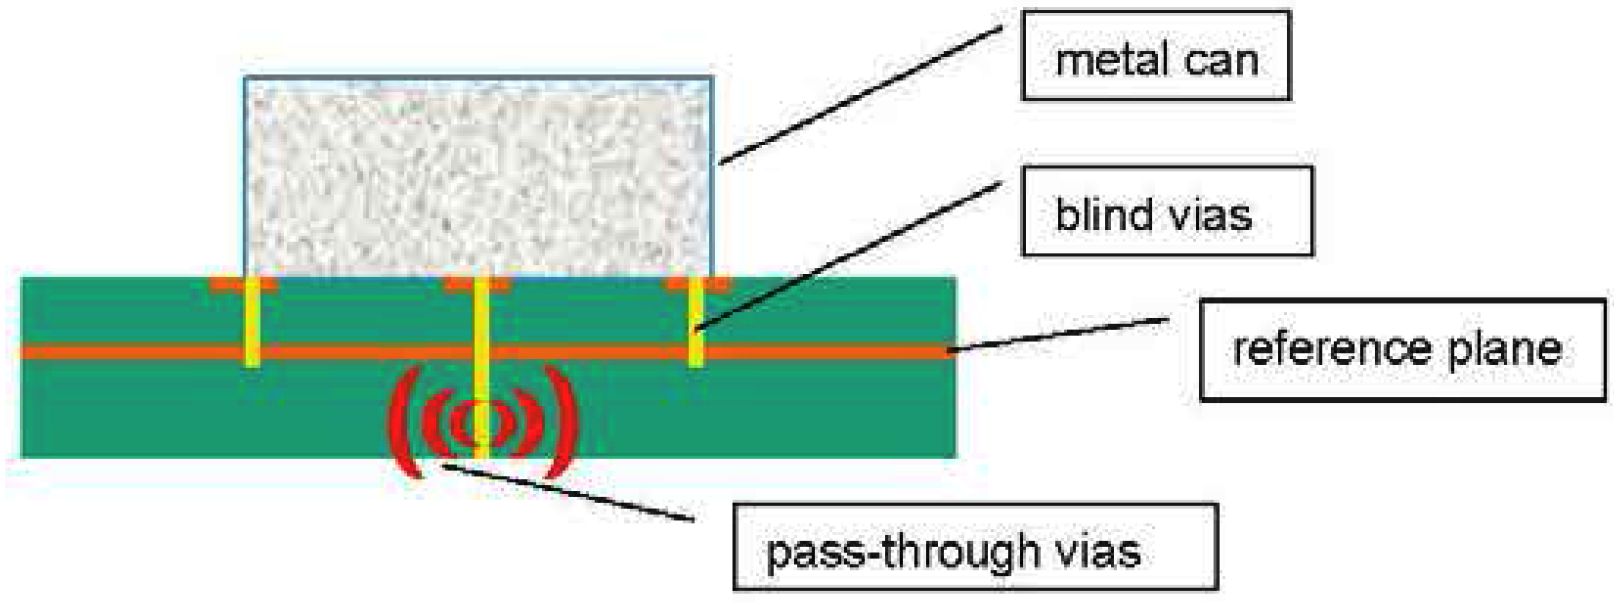
\includegraphics[width=0.5\textwidth]{images/Vias.png}
				\caption{Blind vs. Pass-Through Vias}
				\label{Fig:BlindvsPassthroughVias}
			\end{figure}
			Pass-through vias are short stubs (signal reflections) and emitting antennas, they create holes in the reference plane which reduces its shielding effects!
		\subsubsection{Passing signals across different PCB areas $\rightarrow$ Filtering}
		If different functional areas are considered to be part of the same shielded group the signal traces must be shielded (=inside) as well, this also applies for blocks which are connected through a shielded coax cable. \\
		In all other cases apply adequate filtering:
		\begin{itemize}
			\item Optocouplers are a valid alternative for crossing the boundary of a shielded zone.
			\item Add series L/R to I/O signals going to connectors and avoid GND area under these components to reduce input/output stray capacitance on these elements. 
			\item Add capacitors to the 0V plane and keep these connections very short. Use vias directly to the reference plane. 
			\item At frequencies above 10 MHz replace inductors with ferrite beads. 
			\item Consider using common mode chokes. 
			\item Whenever possible, group all connectors on the same side of the PCB. 
			\item Keep internal signals away from the connector area. 
			\item Keep GND connections of filtering components as short as possible in order to reduce the L. 
		\end{itemize}
		\begin{figure}[h!]
			\centering
			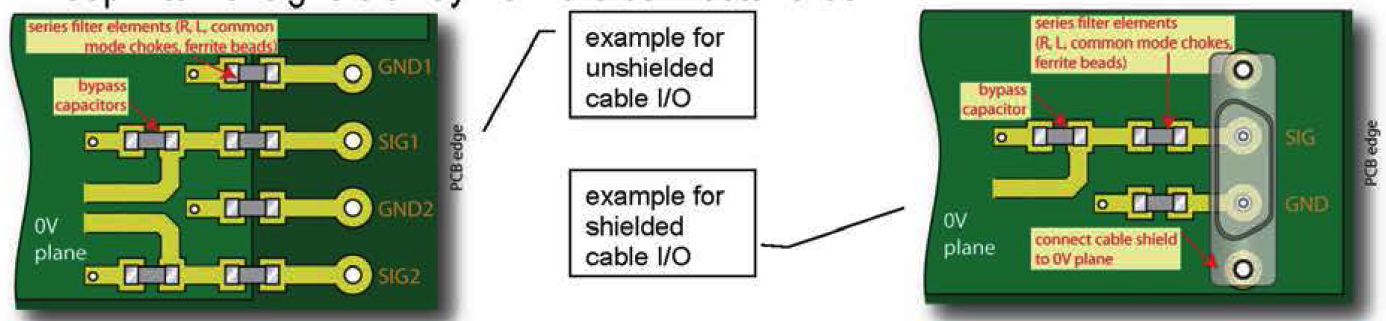
\includegraphics[width=0.65\textwidth]{images/ShieldUnshieldedIO.png}
			\caption{Shield vs. Unshielded connection}
			\label{Fig:ShieldvsUnshielded}
		\end{figure}
		\begin{figure}[h!]
			\centering
			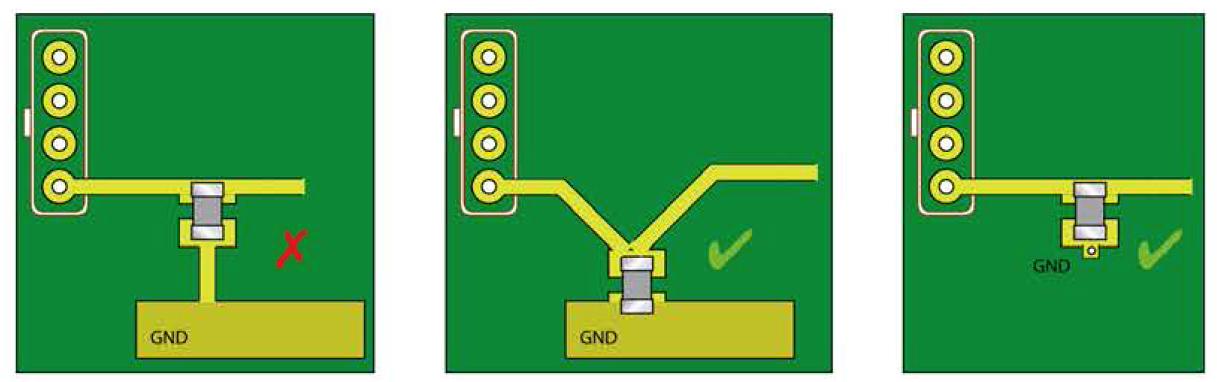
\includegraphics[width=0.65\textwidth]{images/GoodBadConnection.png}
			\caption{Good vs. Bad connection}
			\label{Fig:GoodvsBad}
		\end{figure}
		Heatsinks can cause a problem because they radiate at high frequencies, however, they can be used as the top lid of the shielding can as shown in Figure \ref{Fig:Heatsink}.
		\begin{figure}[h!]
			\centering
			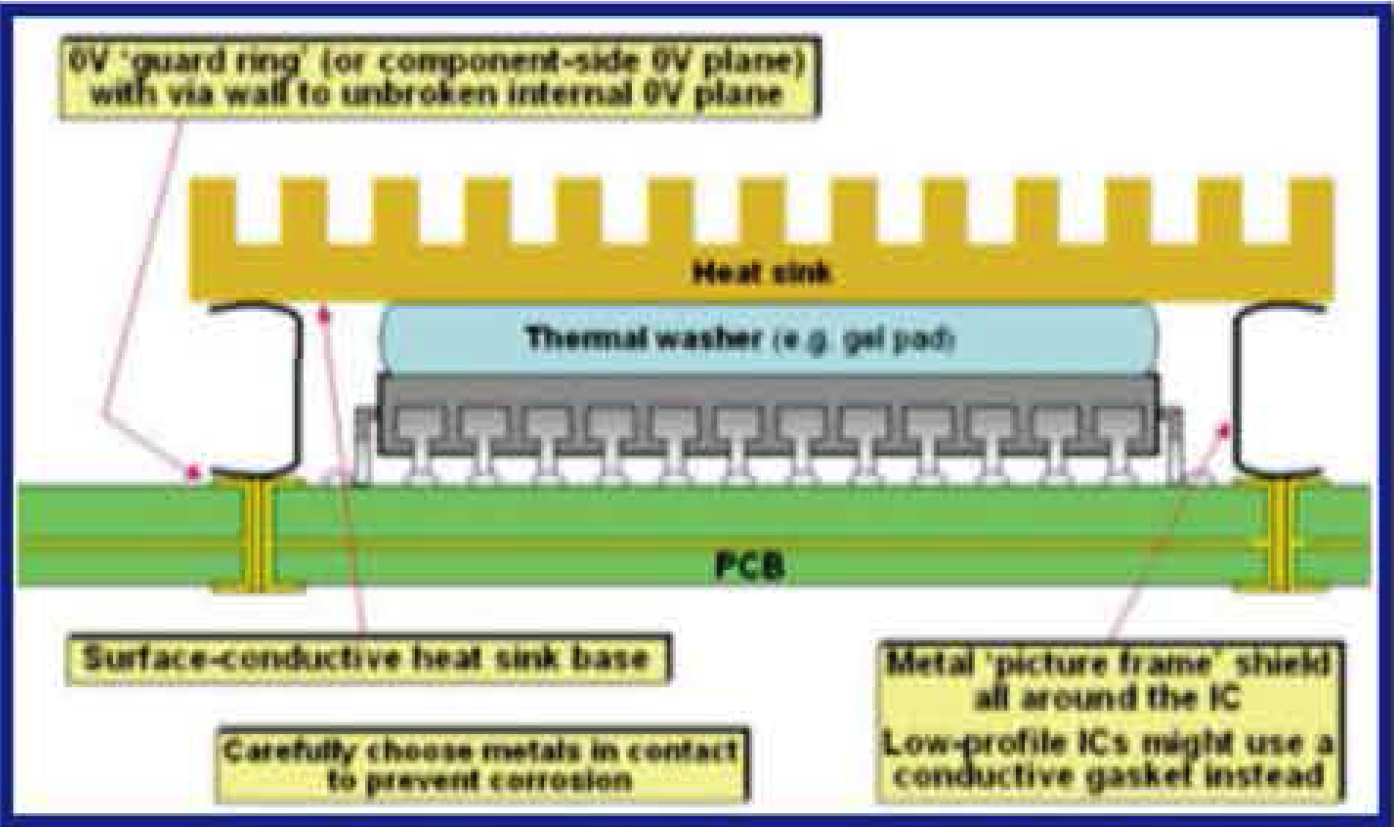
\includegraphics[width=0.5\textwidth]{images/Heatsink.png}
			\caption{Heatsink used as top lid of shielding can}
			\label{Fig:Heatsink}
		\end{figure}	
		\\
		\textbf{Suggested workflow for the PCB design :}
		\begin{itemize}
			\item Use multi-layer PCB and assign two layers the the reference plane (GND, VCC)
			\item Position I/O connectors at the periphery of the PCB under consideration of external cabling layout requirements. This defines the outer world are of the PCB.
			\item Place critical components (high speed interfaces, fast clock circuits sensitive analog circuits) and partition them carefully. Keep them at some distance from I/O connectors. This defines the inner world of the PCB.
			\item Draw reference planes
			\item Place the remaining uncritical components
			\item Route the remaining nets. This is the only task that should be assigned to the autorouter. 
		\end{itemize}
		\subsubsection{Image (Reference) Planes}
		Every signal has a return path, keeping the distance between forward and return path small reduces the loop area which in turn reduces emissions. When an image plane is present, the return current will choose the path forming the smallest loop since this is the solution for the minimal inductance and the minimal stored energy in the magnetic field. The return current in the image plane concentrates directly under the signal trace, where the current density $J$ at a distance x from the centre under the signal trace is:  
		\begin{equation}
			J(x) = \frac{I_0}{\pi h} \cdot \frac{1}{1+\left(\frac{x}{h}\right)^2}
		\end{equation}
		\begin{figure}[h!]
			\centering
			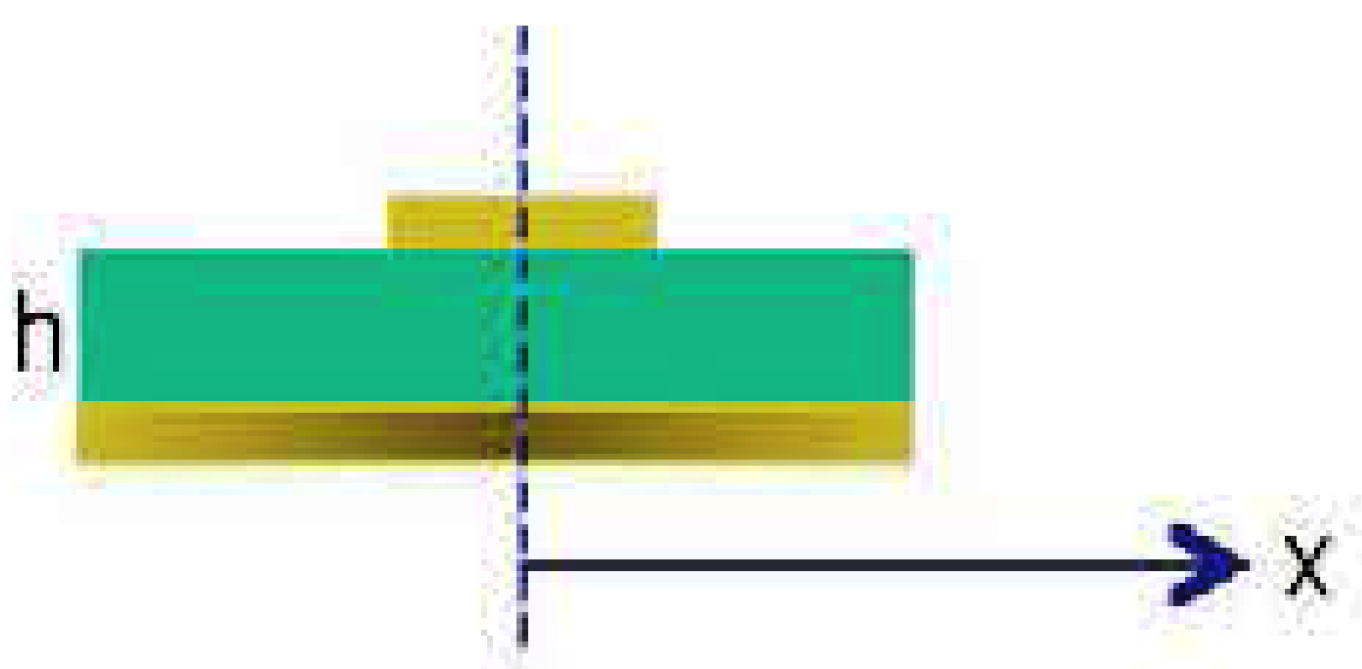
\includegraphics[width=0.25\textwidth]{images/ReturnCurrentGeometry.png}
			\caption{Geometry for return current density}
			\label{Fig:ReturnCurrentGeometry}
		\end{figure}
		\begin{figure}[h!]
			\centering
			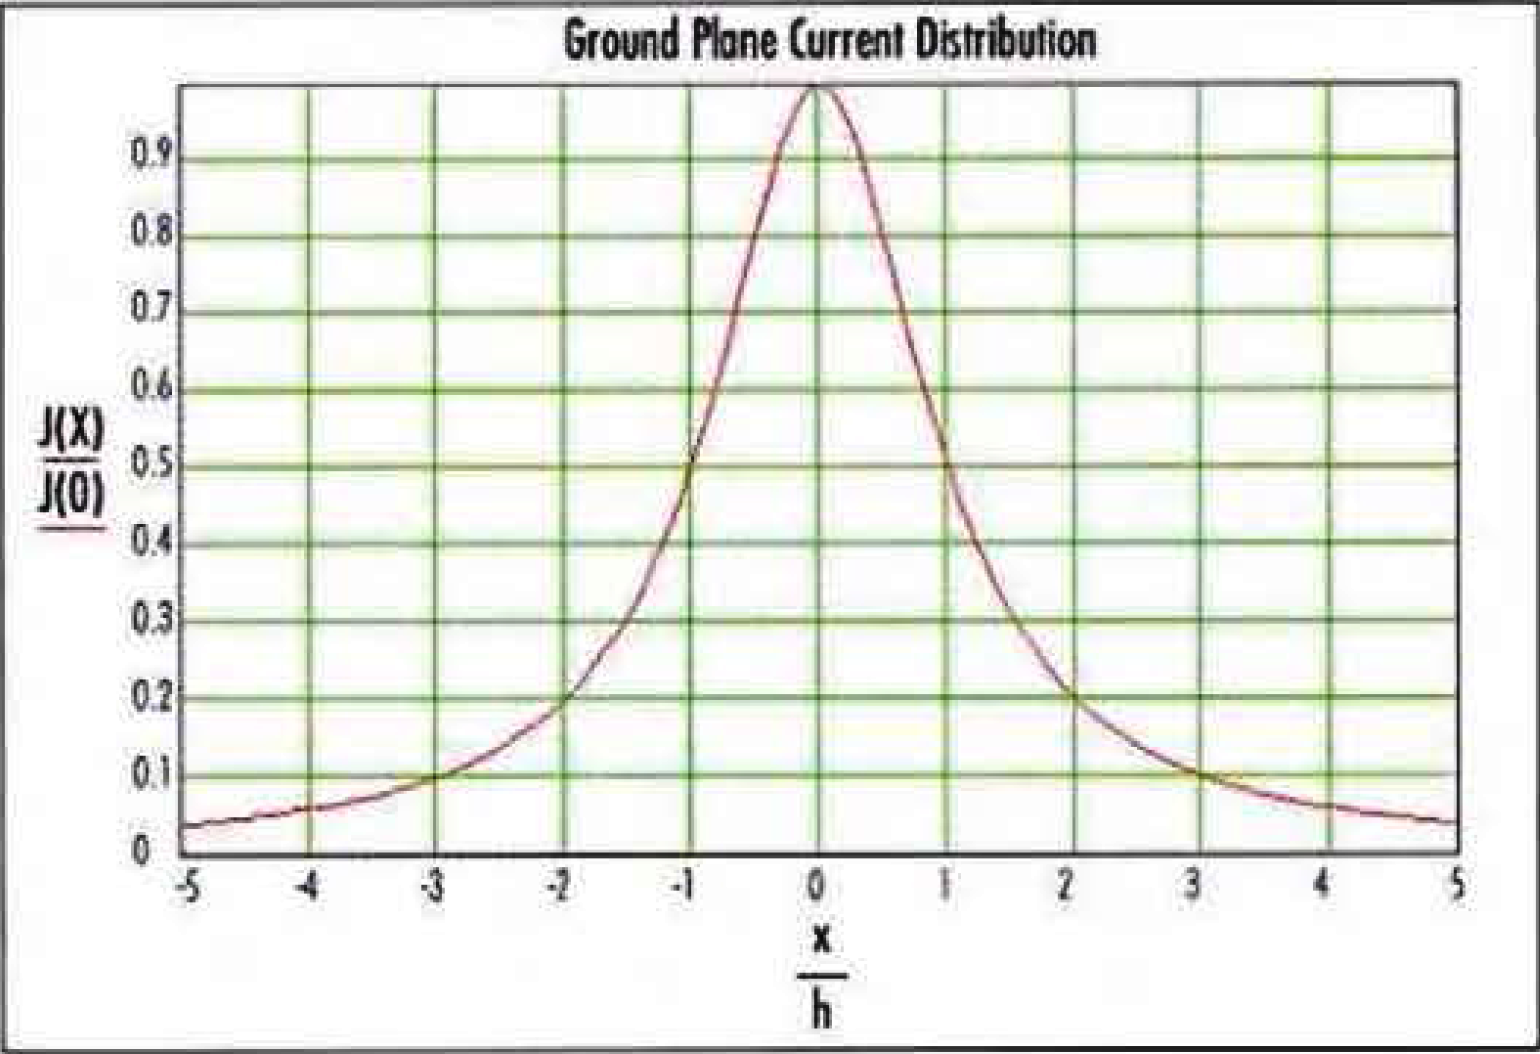
\includegraphics[width=0.4\textwidth]{images/ReturnCurrentDensity.png}
			\caption{Return Current Distribution}
			\label{Fig:ReturnCurrentDensity}
		\end{figure}
		\\
	
		
		\begin{table}[h!]
		\centering
		\begin{tabular}{|m{0.35\textwidth}|m{0.35\textwidth}|}
				\multicolumn{2}{c}{\textbf{Common Mode Noise}}
			\\
			\hline
				Rf field generated by differential mode currents are only a minor part of the problem, because they are confined to small loops (at far field they cancel each other). 
			& 
				 \begin{center}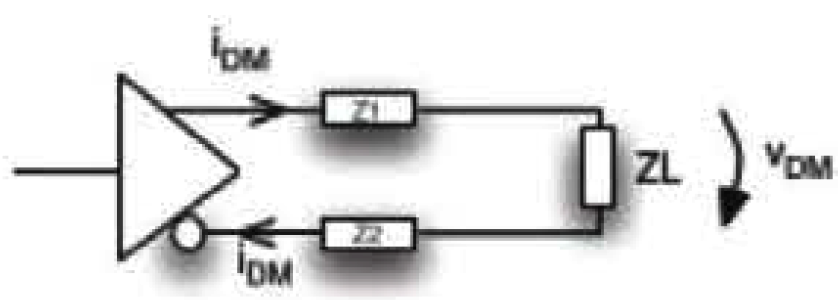
\includegraphics[width=0.35\textwidth]{images/DiffMode.png}\end{center}  
			\\
			\hline
				Common mode currents of smaller amplitude generate much higher emissions since they add at far field. 
			& 
				 \begin{center}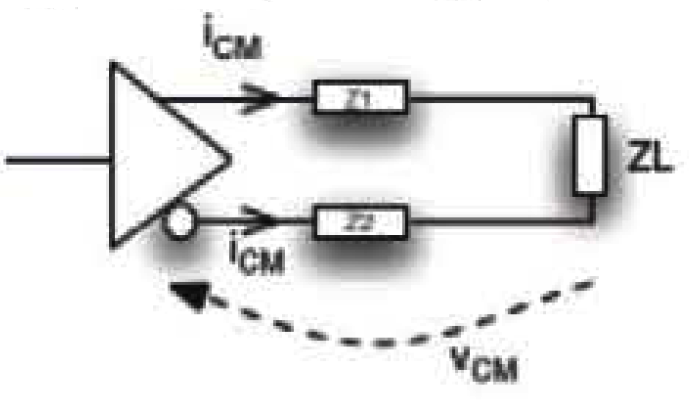
\includegraphics[width=0.35\textwidth]{images/CommonMode.png}\end{center}  
			\\
			\hline
			\end{tabular}
		\end{table}

		\begin{table}[h!]
		\centering
		\begin{tabular}{|m{0.35\textwidth}|m{0.35\textwidth}|}
				\multicolumn{2}{c}{\textbf{Examples of how common mode currents are generated}}
			\\
			\hline
				Consequences of ground noise generated by series impedance in the GND return trace. 
			& 
				 \begin{center}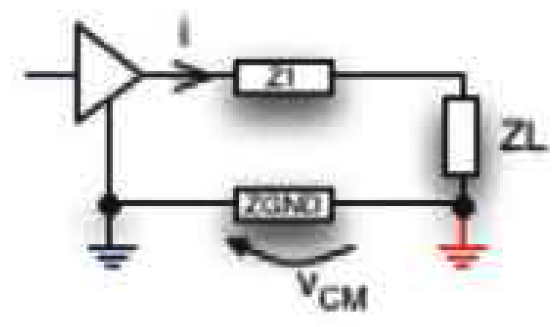
\includegraphics[width=0.35\textwidth]{images/SeriesImpedance.png}\end{center}  
			\\
			\hline
				Even if the return path is not through GND (differential line), different parasitic loading or trace length mismatch can induce common mode currents.  
			& 
				 \begin{center}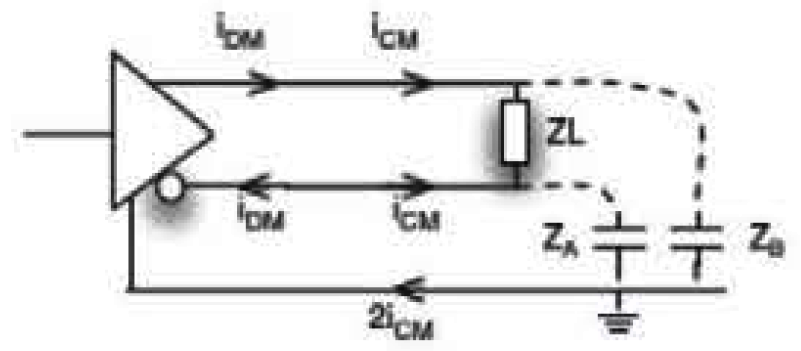
\includegraphics[width=0.35\textwidth]{images/ParasiticLoading.png}\end{center}  
			\\
			\hline
				Noise sources external to the circuit. 
			& 
				 \begin{center}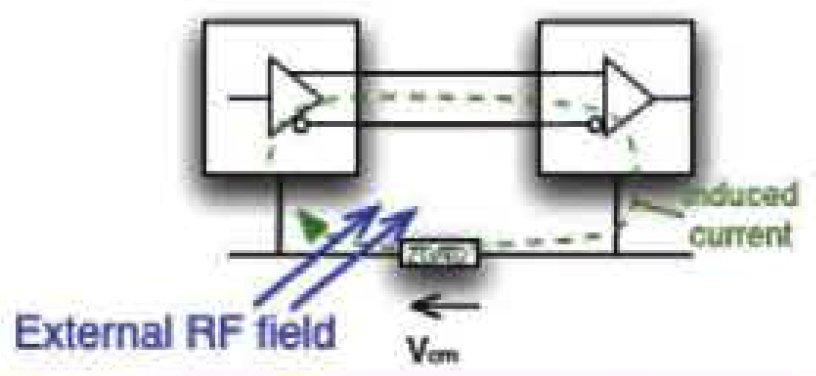
\includegraphics[width=0.35\textwidth]{images/ExternalNoise.png}\end{center}  
			\\
			\hline
			\end{tabular}
		\end{table}


		\begin{table}[h!]
		\centering
		\begin{tabular}{|m{0.35\textwidth}|m{0.35\textwidth}|}
				\multicolumn{2}{c}{\textbf{Why is common mode noise so undesired?}}
			\\
			\hline
				Ground noise can translate to emissions if cables are attached (dipole!). 
			& 
				 \begin{center}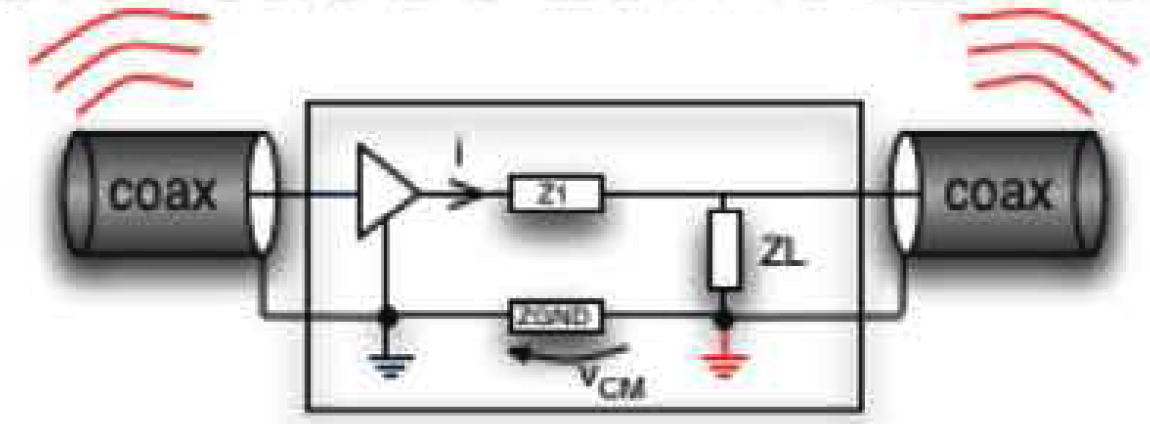
\includegraphics[width=0.35\textwidth]{images/GroundNoiseCables.png}\end{center}  
			\\
			\hline
				Common mode currents can produce unwanted voltages inside the circuit. In the example, when $Z_A \neq Z_B$ then $i_{cm}$ produces a voltage on $Z_L$.
			& 
				 \begin{center}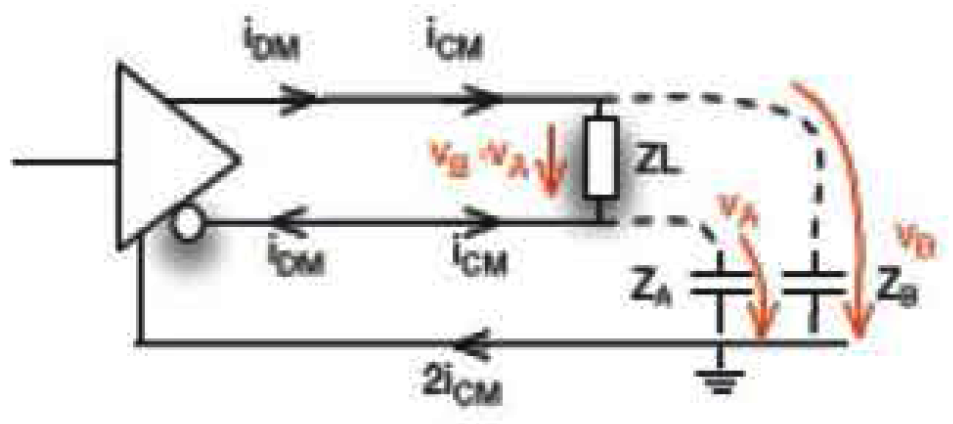
\includegraphics[width=0.35\textwidth]{images/UndesiredVoltages.png}\end{center}  
			\\
			\hline
			\end{tabular}
		\end{table}		
		\clearpage
		\textbf{Common mode currents/voltages in general happen...}
		\begin{itemize}
			\item If the forward and return currents do not cancel out, which happens when the return path is far from the forward path and if they have different lengths, impedances or parasitic load or if there are multiple return paths present. 
			\item If there is a voltage drop in the GND return path ($Z_{GND} \neq 0$)
			\item \textbf{Always provide a return path as close as possible to the forward path, which is best accomplished by a near reference or image plane (GND)}
			\item Mathematical proof that the effective impedance is minimized when forward and return traces are near can be found on the slides page 33 (Week 2).
		\end{itemize}
		
		\begin{table}[h!]
		\centering
		\begin{tabular}{|m{0.35\textwidth}|m{0.35\textwidth}|}
				\multicolumn{2}{c}{\textbf{Image or Reference Plane}}
			\\
			\hline
				\textbf{Stripline Technology}\newline
				Embed signal traces between two image planes (sandwich construction) for best shielding of noisy signals to effectively protect sensitive analog traces against external noise. 
			& 
				 \begin{center}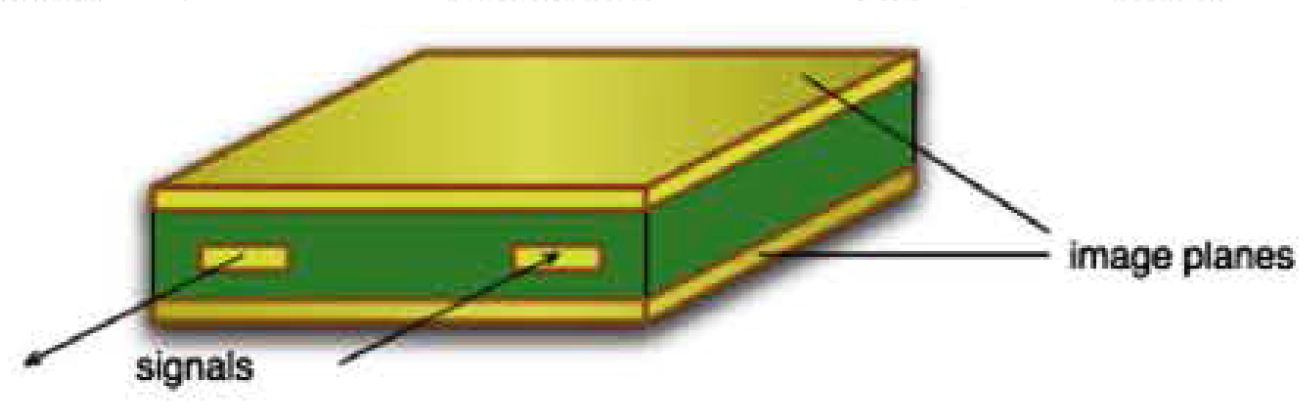
\includegraphics[width=0.35\textwidth]{images/StriplineTechnology.png}\end{center}  
			\\
			\hline
				\textbf{Microstrip Technology}\newline
				This is the most commonly used technology. It is a little less effective than stripline however.  
			& 
				 \begin{center}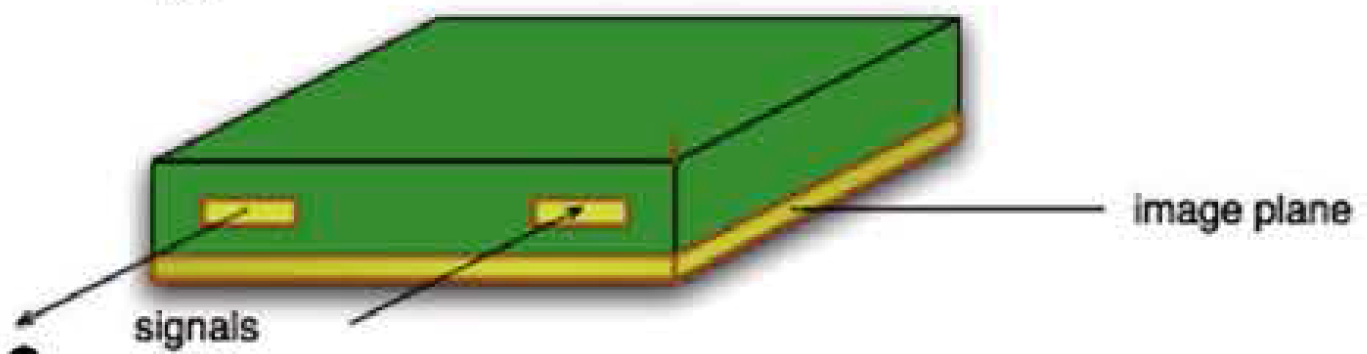
\includegraphics[width=0.35\textwidth]{images/MicrostripTechnology.png}\end{center}  
			\\
			\hline
				\multicolumn{2}{c}{\textbf{Both GND and VCC can be used. VCC however is generally more noisy than GND.}}
			\\
			\hline
				Example of reference planes in multilayer PCB (see other examples on slide 35 from Week 2) 
			& 
				 \begin{center}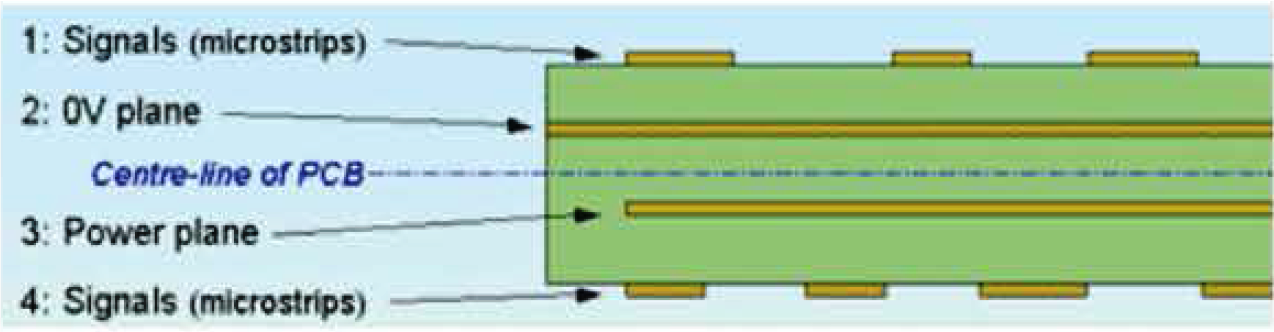
\includegraphics[width=0.5\textwidth]{images/ExampleReferenceLayer.png}\end{center}  
			\\
			\hline
			\end{tabular}
		\end{table}	
		
		\subsubsection{To split or not to split the ground plane}
		Literature is quite discordant on this subject, up to 10-15 years ago partitioning the GND plane was a recommended practice. However, today the specialists tend to agree that this should be done only in very special circumstances (e.g. isolation required) and under advice of an EMC expert. 		
		Most recent publications and app notes suggest not to split the GND plane:
		\begin{itemize}
			\item A well-designed GND plane on its own layer in a PCB is possibly the most cost-effective EMC design technique that has ever existed or ever will. 
			\item The use of plane cuts, reference plane discontinuities, is one of the most widespread contributors to EMC occurrences that we see. 
		\end{itemize}
		Why splitting can be a bad choice: 
		\begin{itemize}
			\item Every signal has its own return path. Typically the return path finds its way in the GND plane just under the signal trace. Voiding or Splitting the plane forces the return path to take a detour. 
			\item Forward and backward path form a loop. Increasing the loop area inevitably increases its HF radiation (loop antenna).
			\item Planes having a HF voltage difference act as a dipole antenna! 
			\item Do not void a reference plane just to route a signal, always think of the return paths!
			\item See slide 41 from Week 2 for bad examples of GND planes!
		\end{itemize}

		
		\begin{table}[h!]
		\centering
		\begin{tabular}{|m{0.35\textwidth}|m{0.35\textwidth}|}
				\multicolumn{2}{c}{\textbf{Some examples for splitting the GND plane}}
			\\
			\hline
				Separate GND for sensitive analog circuitry from noisy digital. 
			& 
				 \begin{center}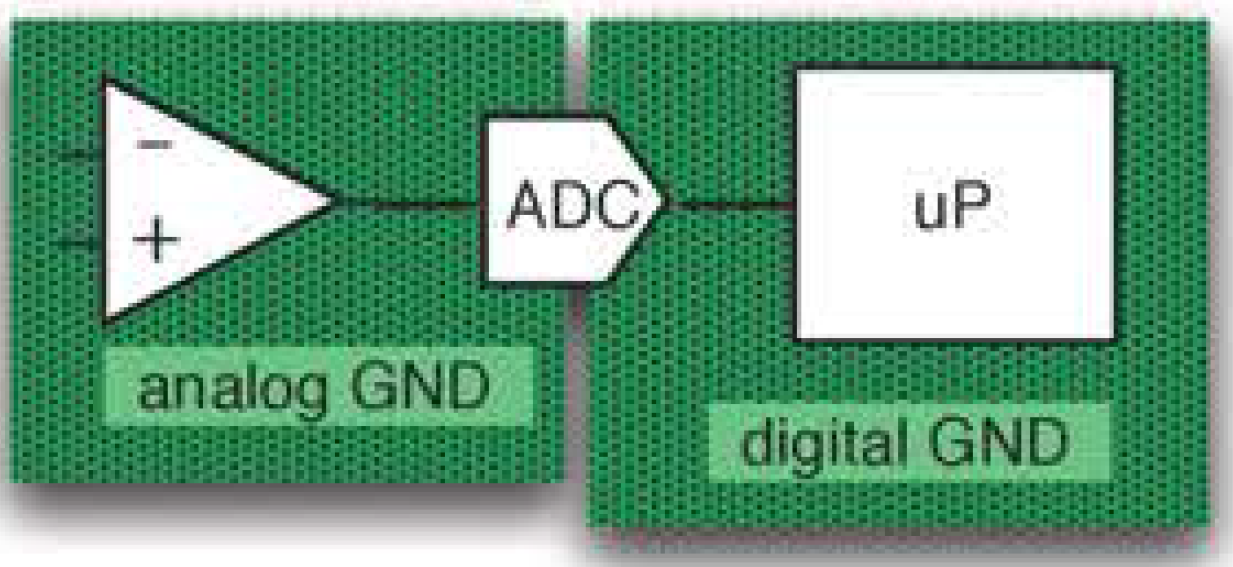
\includegraphics[width=0.35\textwidth]{images/GNDSep1.png}\end{center}  
			\\
			\hline
				Separate GND fro I/O signals.
			& 
				 \begin{center}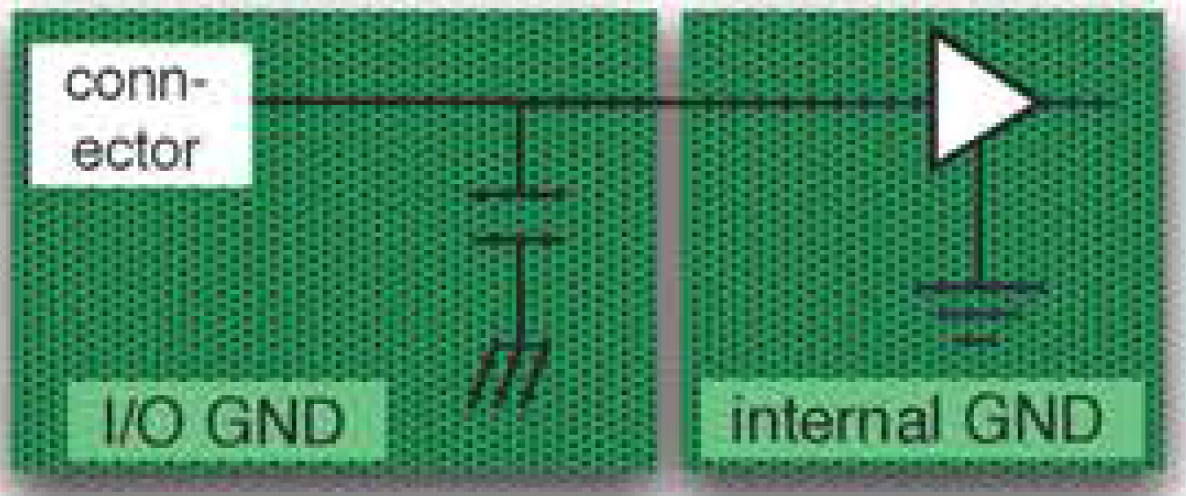
\includegraphics[width=0.35\textwidth]{images/GNDSep2.png}\end{center}  
			\\
			\hline
				Separate high-speed oscillators from the rest of the circuitry. 	
			& 
				 \begin{center}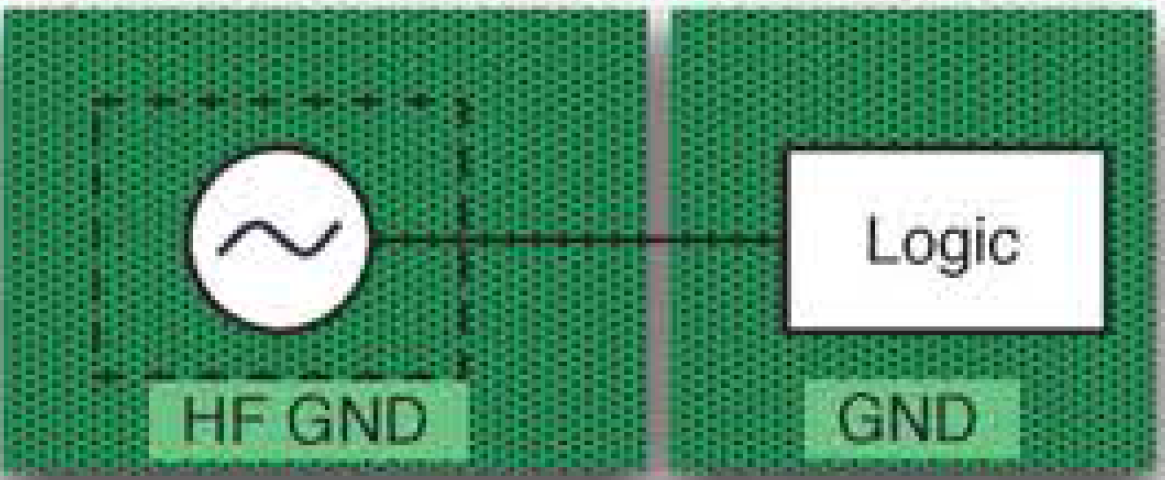
\includegraphics[width=0.35\textwidth]{images/GNDSep3.png}\end{center}  
			\\
			\hline
			\end{tabular}
		\end{table}	
		\begin{table}[h!]
		\centering
		\begin{tabular}{|m{0.45\textwidth}|m{0.35\textwidth}|}
				\multicolumn{2}{c}{\textbf{Electromagnetic field radiated by small current loop and small dipole antenna}}
			\\
			\hline
				In the main radiating direction, a PCB trace carrying a current $I$ and forming a loop of area $A$ generates an electromagnetic field at a point distant $R$ in the order of:\newline
				\begin{equation}
					E \sim \frac{k^2 I A}{4\pi} \sqrt{\frac{\mu}{\varepsilon}}\frac{1}{R}
				\end{equation}
				\begin{equation}
					H \sim \frac{k^2 I A}{4\pi}\frac{1}{R}
				\end{equation}
				where\newline
				$I$ = Current\newline
				$A$ = Loop area\newline
				$R$ = Distance of the measuring point \newline
				$k = \frac{2\pi}{\lambda} = \frac{\omega}{c}$ 
			& 
				 \begin{center}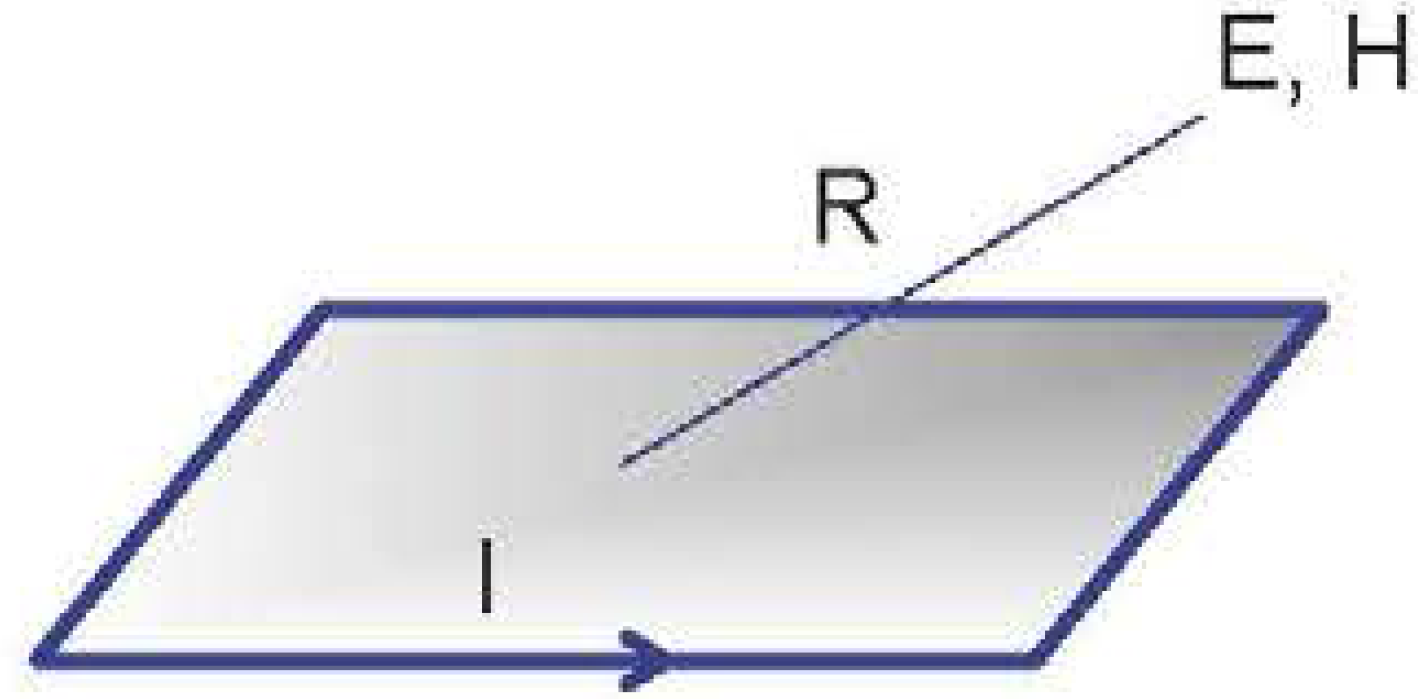
\includegraphics[width=0.35\textwidth]{images/CurrentLoop.png}\end{center}  
			\\
			\hline
				In the main radiating direction, a small dipole antenna fed by a current $I$ and having a length $L$ generates an electromagnetic field at a point distant $R$ in the order of: \newline
				\begin{equation}
					E \sim \frac{I L f}{4\varepsilon_0 R}
				\end{equation}
				where\newline
				$I$ = Current\newline
				$L$ = Length of the dipole\newline
				$R$ = Distance of the measuring point \newline
				$f$ = Frequency of the current				
			& 
				 \begin{center}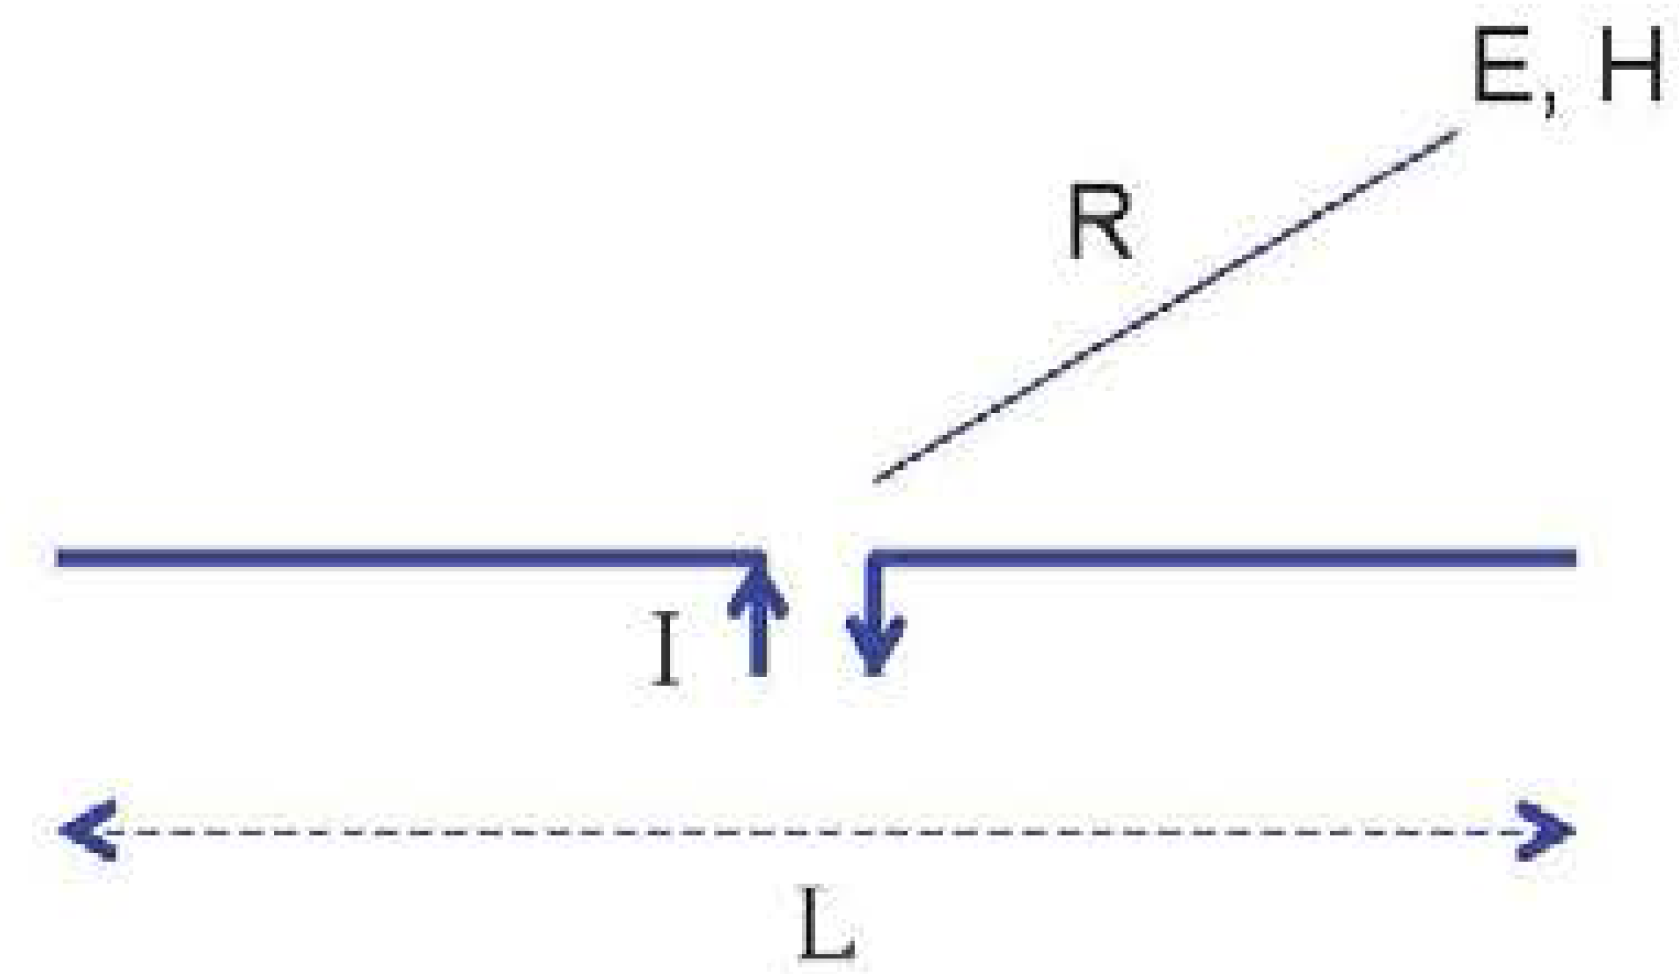
\includegraphics[width=0.35\textwidth]{images/DipoleAntenna.png}\end{center}  
			\\
			\hline
			\end{tabular}
		\end{table}	
		
		\begin{table}[h!]
		\centering
		\begin{tabular}{|m{0.5\textwidth}|m{0.35\textwidth}|}
				\multicolumn{2}{c}{\textbf{Possible Issues with continuous reference planes}}
			\\
			\hline
				\begin{itemize}
					\item If we are unlucky we could excite the resonant frequency of the plane (patch antenna) 
					\item If we have more planes (GND, power) in a multilayer PCB, resonance can build up between them. 
					\item The resonant field between two planes can escape along the PCB edges. 
					\item Beware of slot antennas, which are an inverted dipole with equivalent radiation characteristics. It can be excited by a voltage source or an electromagnetic field, any interruption in a reference plane is a potential slot antenna, when a signal trace carrying an AC signal crosses over/under it. 
					\item Avoid accidental critical interruption of reference planes
					\begin{itemize}
						\item Do not place antipads too close together.
						\item Reduce the number of vias crossing but not contacting the reference plane. 
						\item Reduce the number of THT components. 
					\end{itemize}
				\end{itemize}
			& 
				 \begin{center}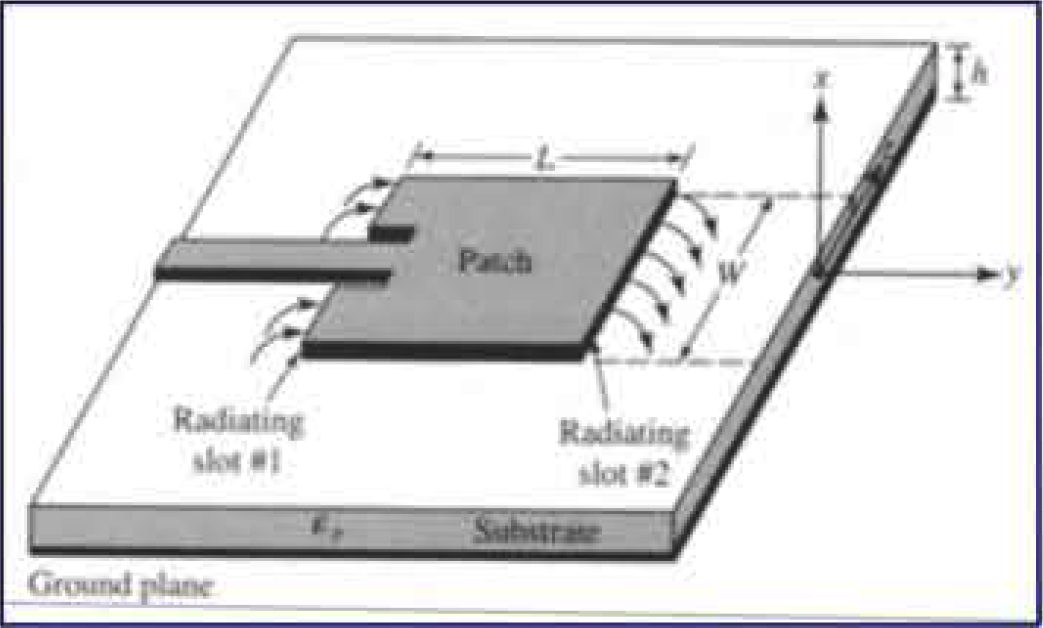
\includegraphics[width=0.35\textwidth]{images/Patchantenna.png}\end{center} 
				 \begin{center}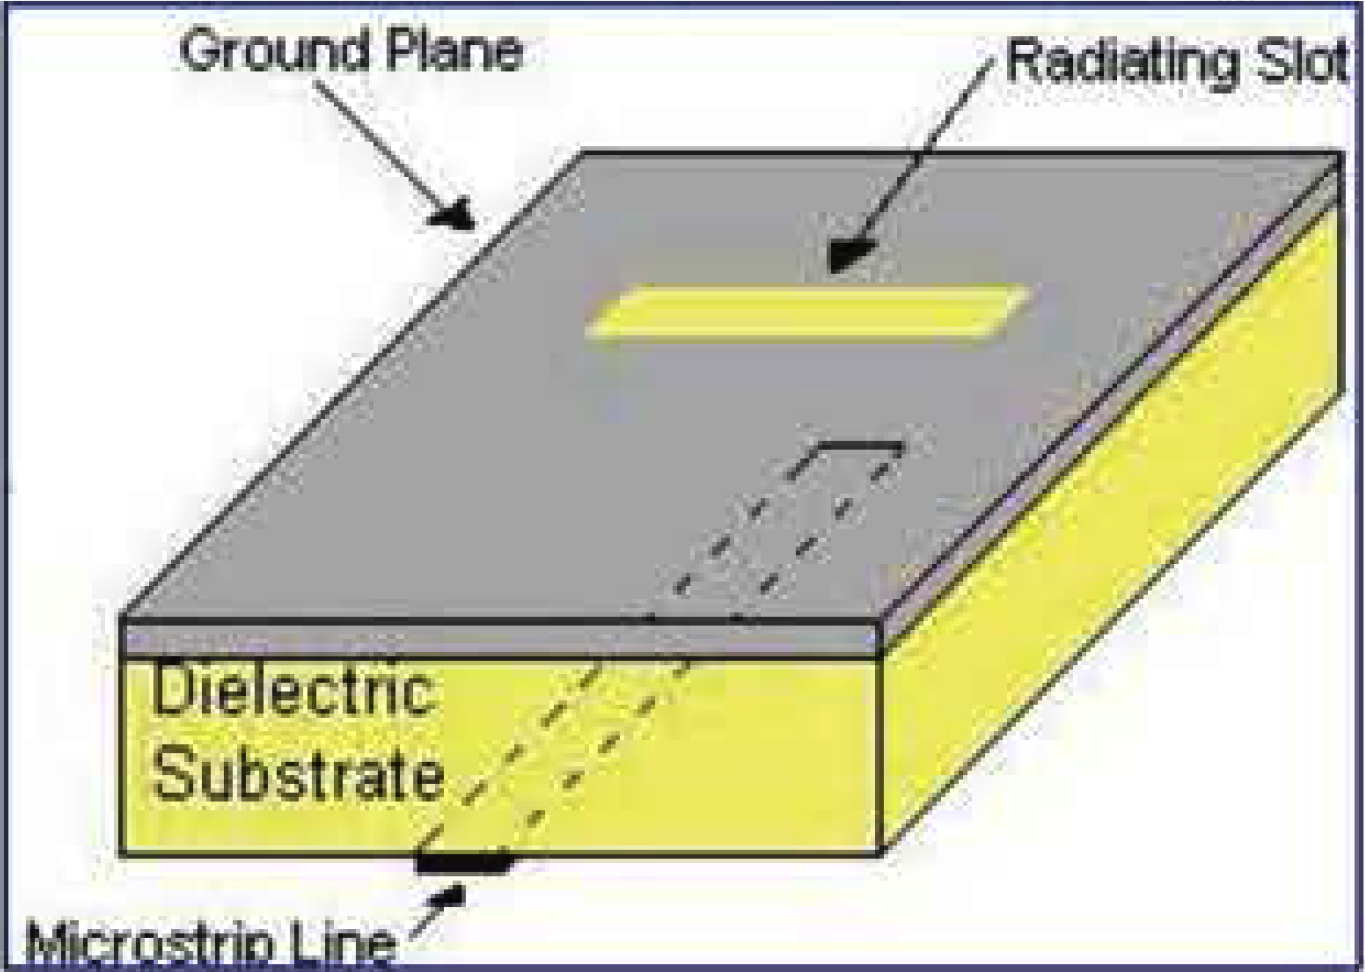
\includegraphics[width=0.35\textwidth]{images/SlotAntenna.png}\end{center} 
				 \begin{center}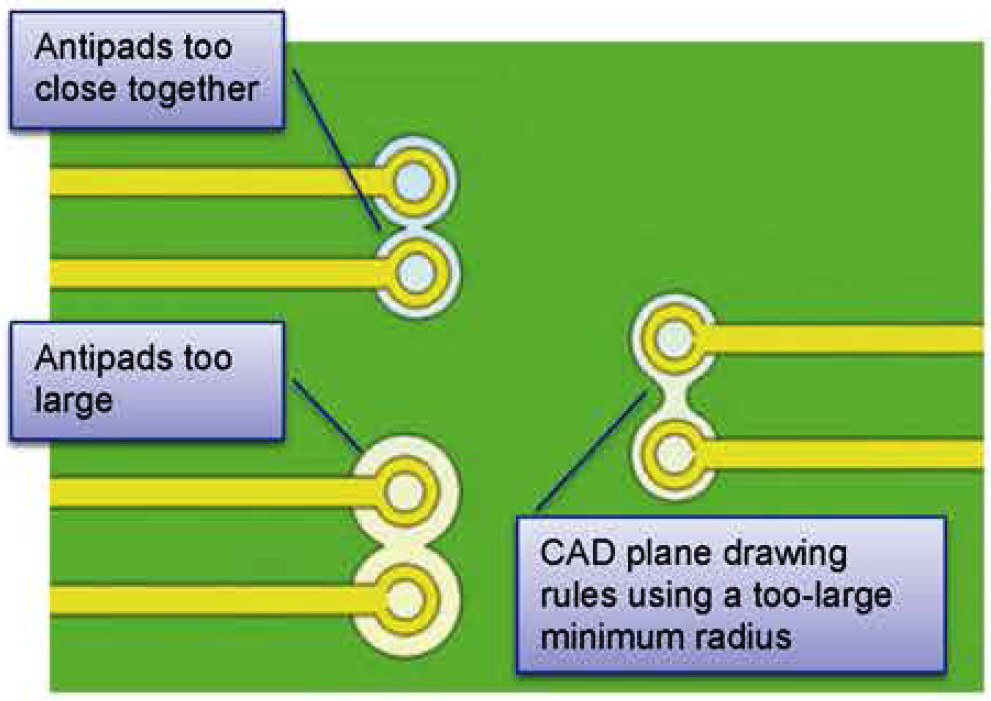
\includegraphics[width=0.35\textwidth]{images/BadAntipads.png}\end{center} 
				 \begin{center}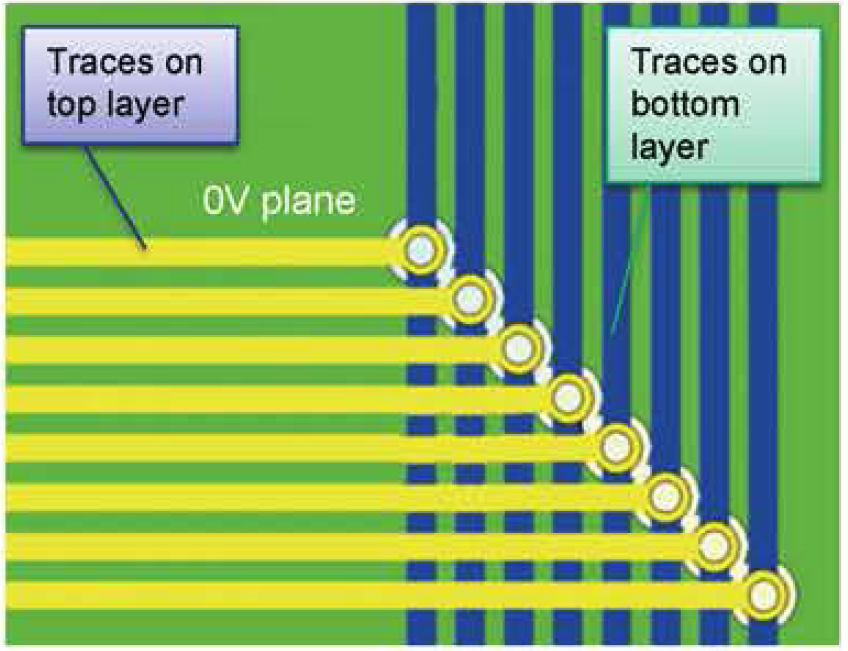
\includegraphics[width=0.35\textwidth]{images/Traces.png}\end{center} 
			\\
			\hline
			\end{tabular}
		\end{table}	

		
		\begin{table}[h!]
		\centering
		\begin{tabular}{|m{0.45\textwidth}|m{0.35\textwidth}|}

				\multicolumn{2}{c}{\textbf{Countermeasures}}
			\\
			\hline
				\begin{itemize}
					\item Put many vias at short distance ($\lambda/10$) to contact the various GND planes. 
					\item Put many bypass capacitors or some shunt resistors between GND and power planes. 
					\item To avoid fringing from the PCB edges, put a GND guard ring on the top and bottom layer and connect them with many vias to block emission. 
				\end{itemize}
			& 
				 \begin{center}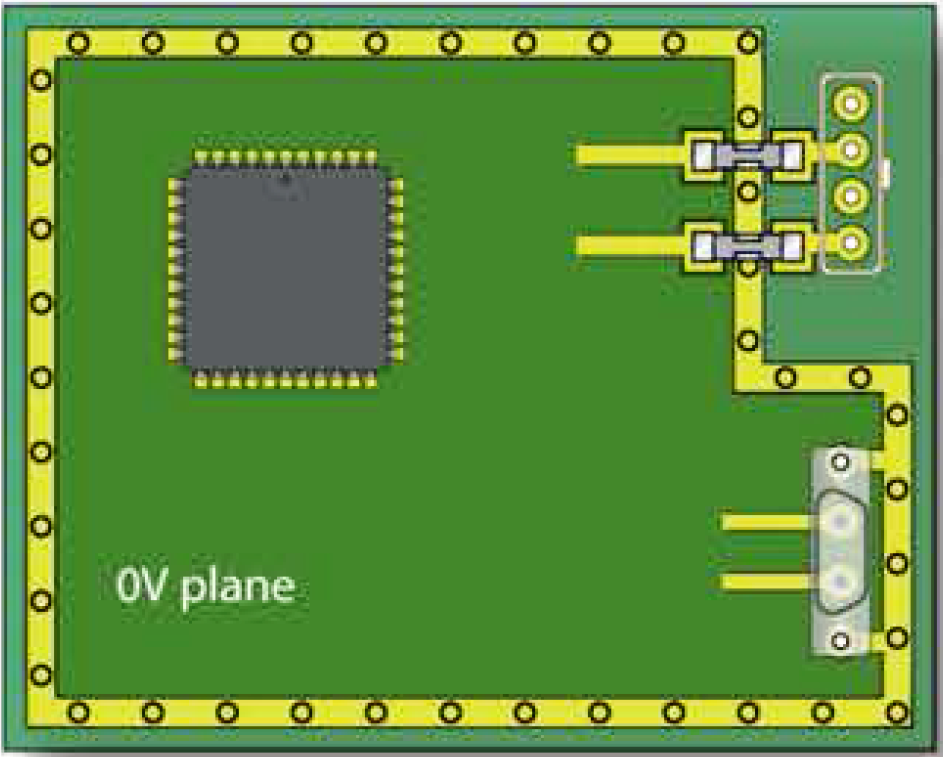
\includegraphics[width=0.35\textwidth]{images/GNDGuard.png}\end{center}  		
			\\
			\hline
			\multicolumn{2}{c}{\textbf{A widespread solution for I/O sections}}
			\\
			\hline
				\begin{itemize}
					\item Shunt HF noise captured by I/O cables to the metal cabinet with the shortest possible path.  
					\item Always provide a nearby signal return path also in the I/O cable. 
				\end{itemize}
			& 
				 \begin{center}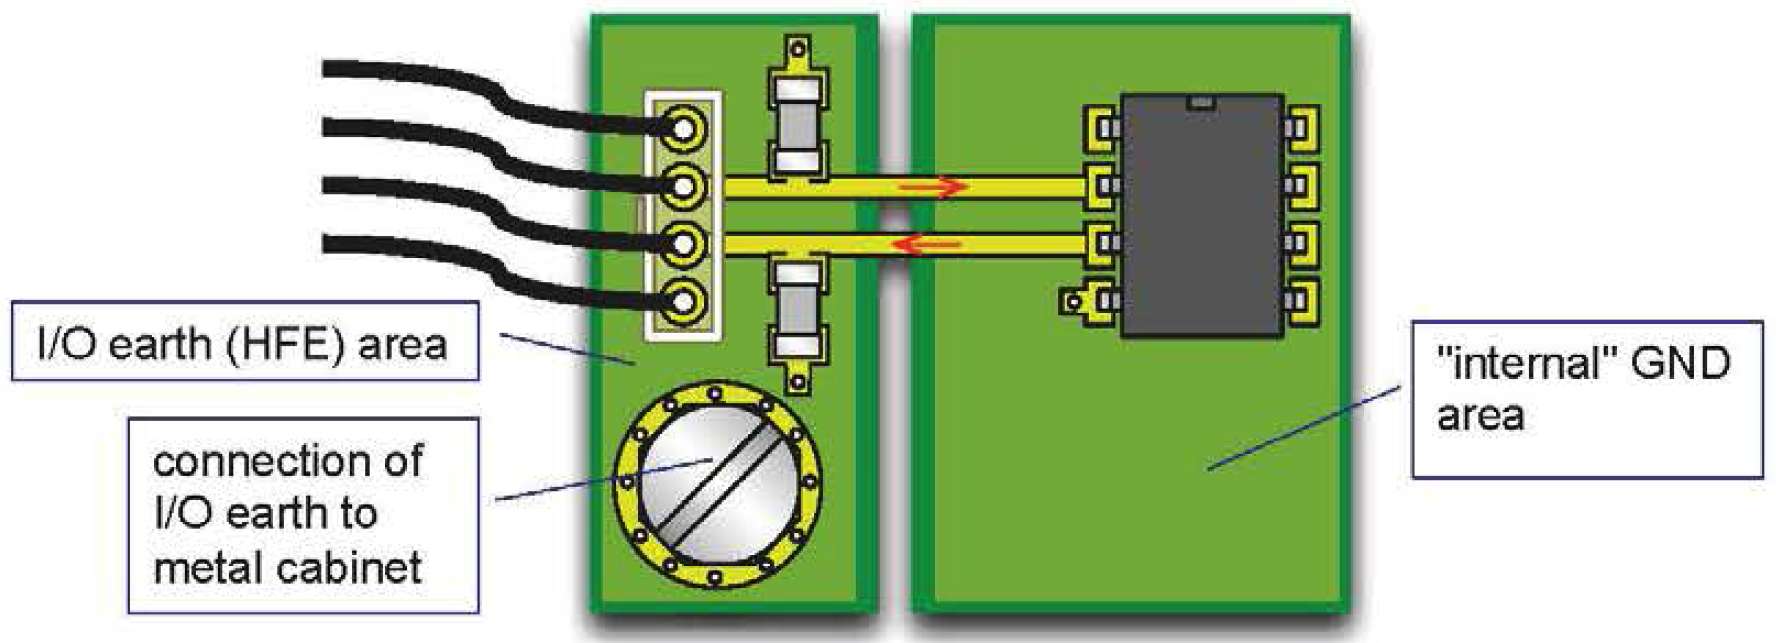
\includegraphics[width=0.35\textwidth]{images/IOSections.png}\end{center}  		
			\\
			\hline
			\end{tabular}
		\end{table}	
		
		\textbf{A few situations where we may still want to split the planes:}
		\begin{itemize}
			\item We want to control where a particular return current travels or where it should never go
			\begin{itemize}
				\item Very high impedance analog circuits
				\item Very small currents (sensor signal conditioning circuits) at DC or very low frequencies
				\item Outputs connected to very noisy, high power (electromechanical) equipment
			\end{itemize}
			\item Isolation needed (safety):Optocoupler circuits
			\item Reduction of parasitic C to GND in filters, line transformers
			\item Consider connecting the different reference planes with a number of small capacitors. They do not influence the low frequency behaviour but help reduce the HF emissions due to differential mode noise between the planes. 
		\end{itemize}
		\clearpage
		\subsubsection{Mixed Signal Circuits}
				\begin{table}[h!]
				\centering
				\begin{tabular}{|m{0.45\textwidth}|m{0.35\textwidth}|}
					\hline
						\begin{itemize}
							\item Manufacturers of mixed signal components often suggest to implement split GND planes (AGND, DGND) in order to avoid having digital noise on the analog signal. 
							\item Analog Devices suggest connecting the two GND via anti-parallel Schottky diodes or ferrite beads. 
						\end{itemize}
					& 
						 \begin{center}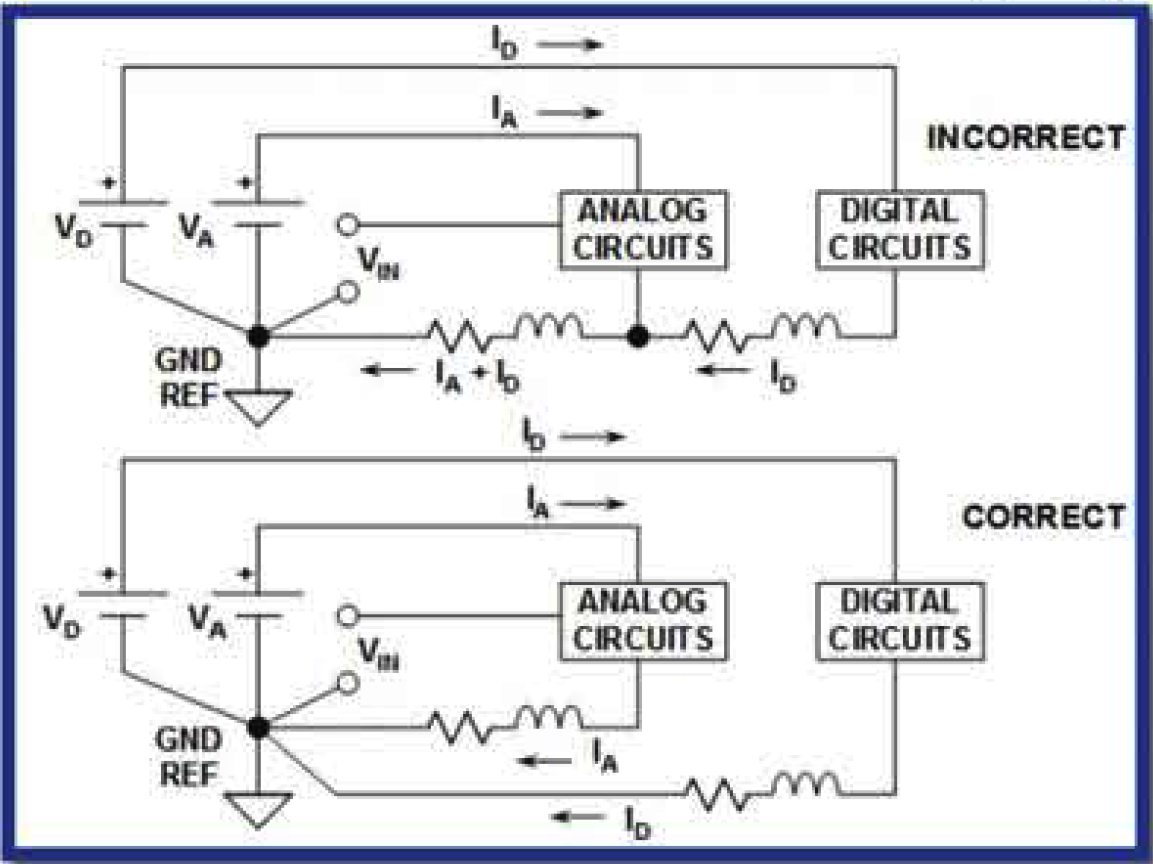
\includegraphics[width=0.35\textwidth]{images/AGND_DGND.png}\end{center}  
						 \begin{center}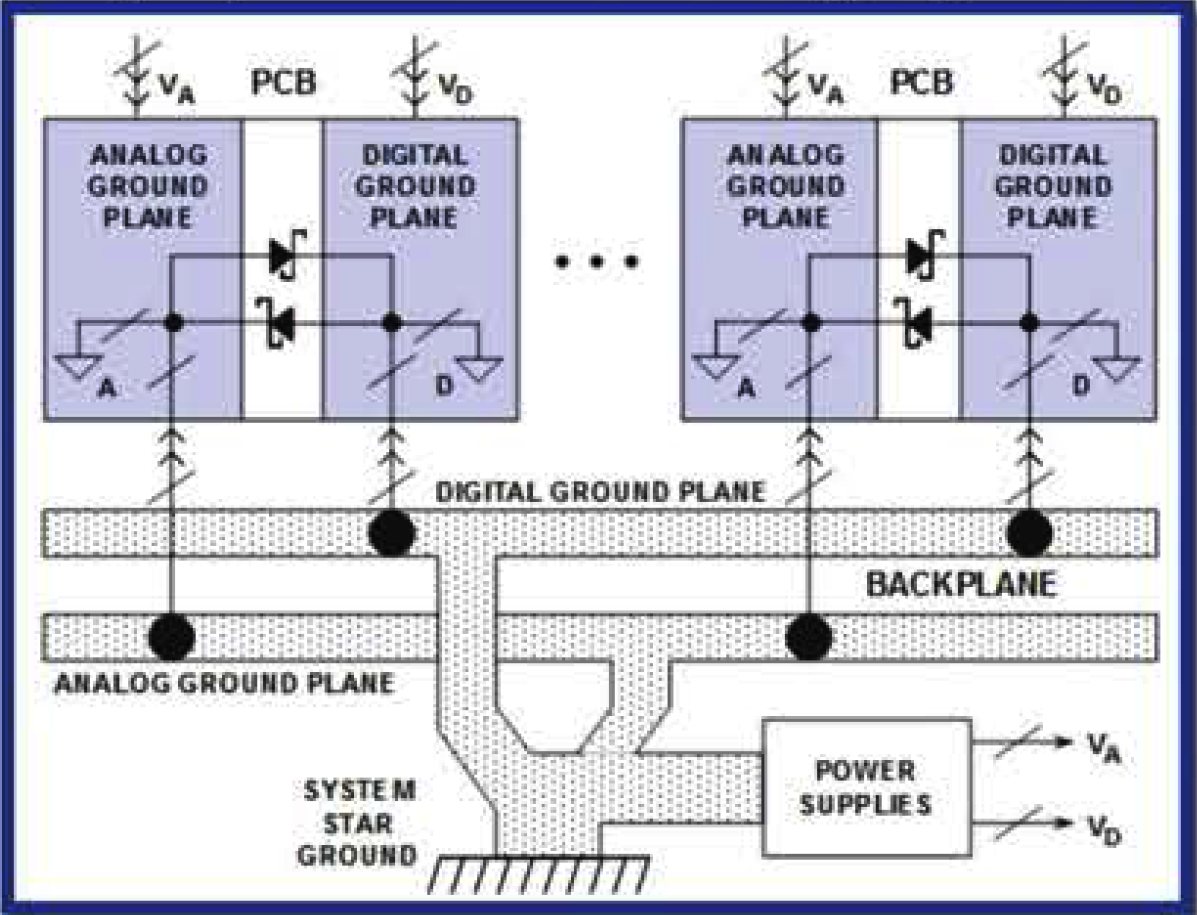
\includegraphics[width=0.35\textwidth]{images/Schottky.png}\end{center}		
					\\
					\hline
						\begin{itemize}
							\item Many A/D, D/A converters have separated analog and digital GND supply pins, generally this is only for practical reasons, because internal bonding has $L \neq 0$ and therefore with a single GND pin, digital noise would couple into the analog section. 
							\item Externally we can tie them together at AGND in most cases.  
						\end{itemize}
					& 
						 \begin{center}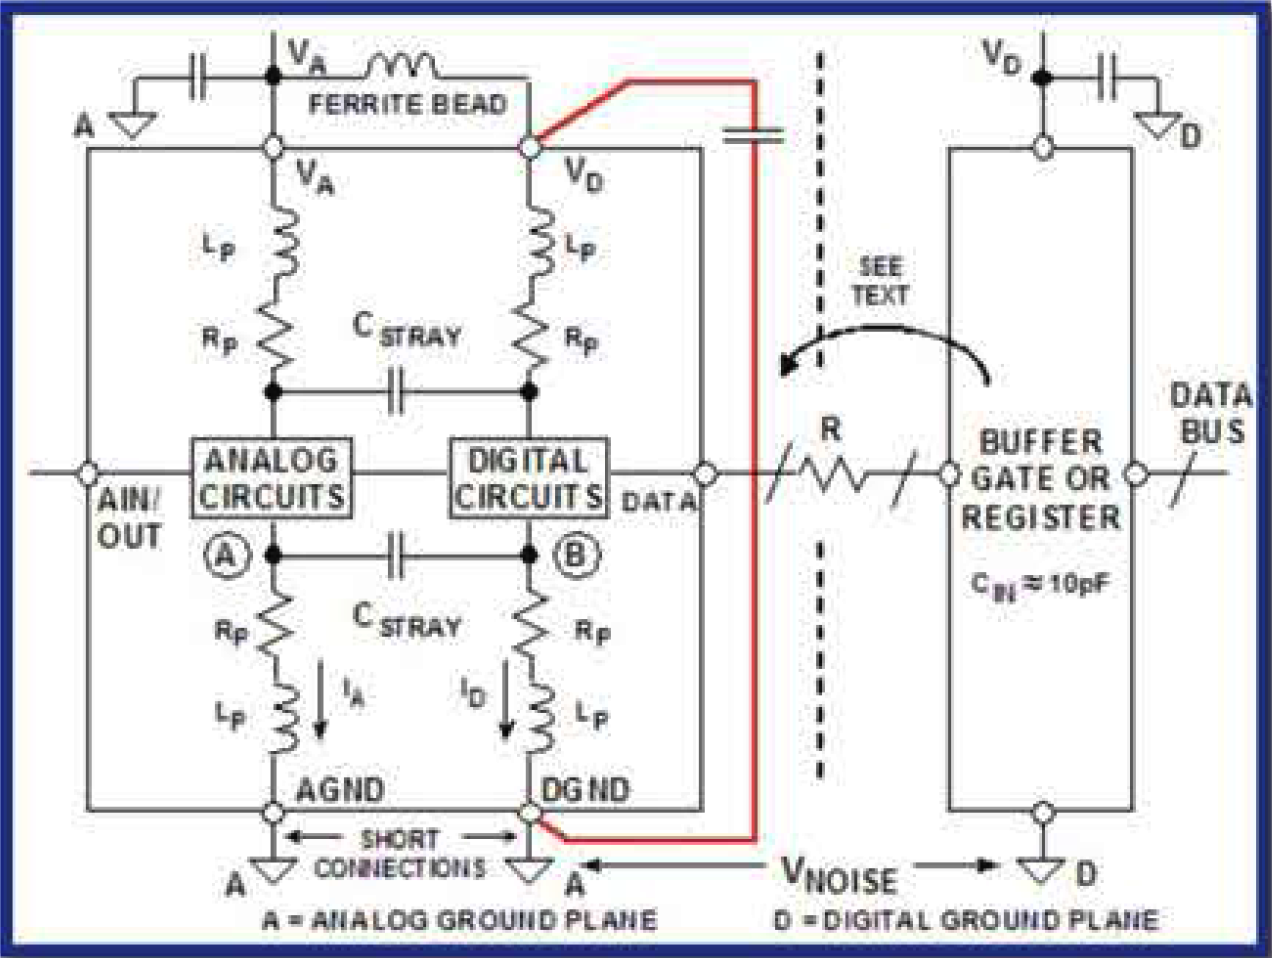
\includegraphics[width=0.35\textwidth]{images/MixedSignal1.png}\end{center}  		
					\\
					\hline
					\end{tabular}
				\end{table}	
				
				\begin{table}[h!]
				\centering
				\begin{tabular}{|m{0.45\textwidth}|m{0.35\textwidth}|}

						\multicolumn{2}{c}{\textbf{Mixed signal ICs with low digital currents}}
					\\
					\hline
						\begin{itemize}
							\item Connect AGND and DGND pins together to the analog reference plane (the IC is located completely in the analog part, see upper Figure), or place it over a star connection point between AGND and DGND (if we have only one ADC, see lower Figure).
							\item Further decouple the AVCC with a ferrite bead and its own decoupling capacitor. 
							\item To further reduce noise consider adding a digital buffer IC on the digital interface
							\begin{itemize}
								\item Decouple noise from the digital bus, the buffer is connected to DGND
								\item The buffer reduces loading (current drawn) on the digital outputs of the ADC. Use series resistors to further reduce the current. 
							\end{itemize}
						\end{itemize}
					& 
						 \begin{center}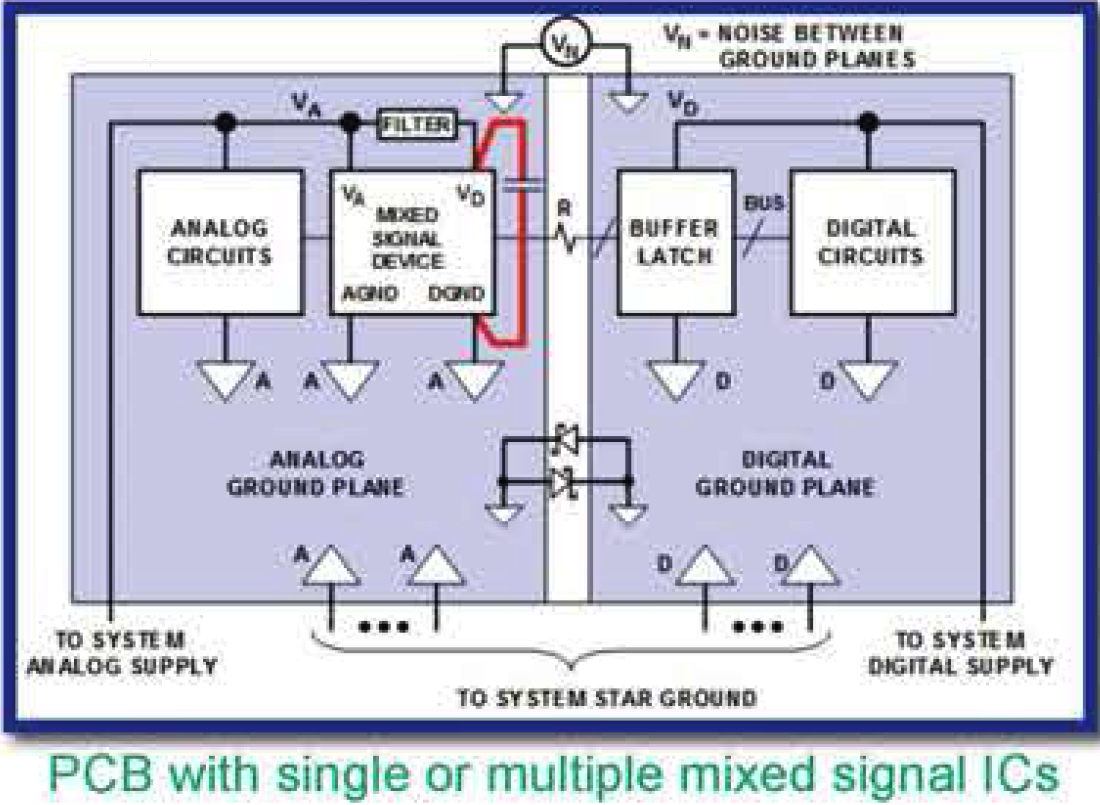
\includegraphics[width=0.35\textwidth]{images/MixedSignal2.png}\end{center}  
						 \begin{center}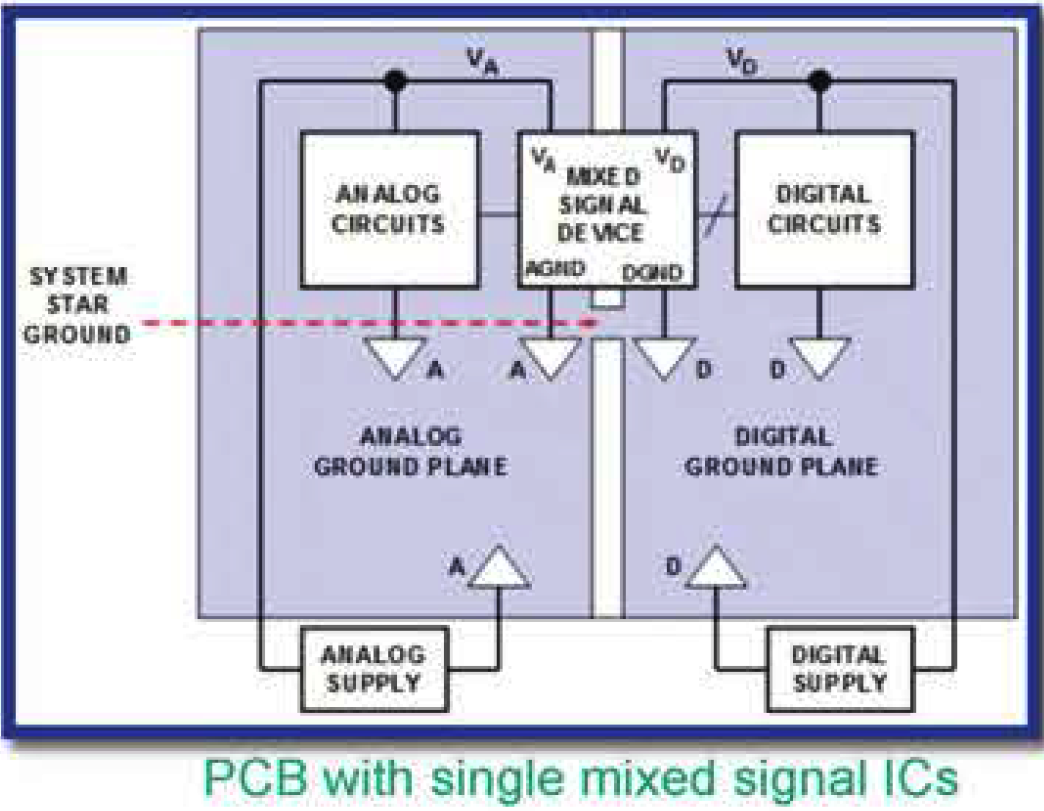
\includegraphics[width=0.35\textwidth]{images/MixedSignal3.png}\end{center}
					\\	
					\hline
						\multicolumn{2}{c}{\textbf{Mixed signal ICs with high digital currents and/or multicard systems}}	
					\\
					\hline
						\begin{itemize}
							\item Connect AGND and DGND pins to the respective reference plane (upper Figure). 
							\item This scheme works only for ICs designs with well isolated analog/digital circuits. 
							\item Tie AGND and DGND together in a star point. In multicard systems this can be at the backplane (lower Figure).
						\end{itemize}
					& 
						 \begin{center}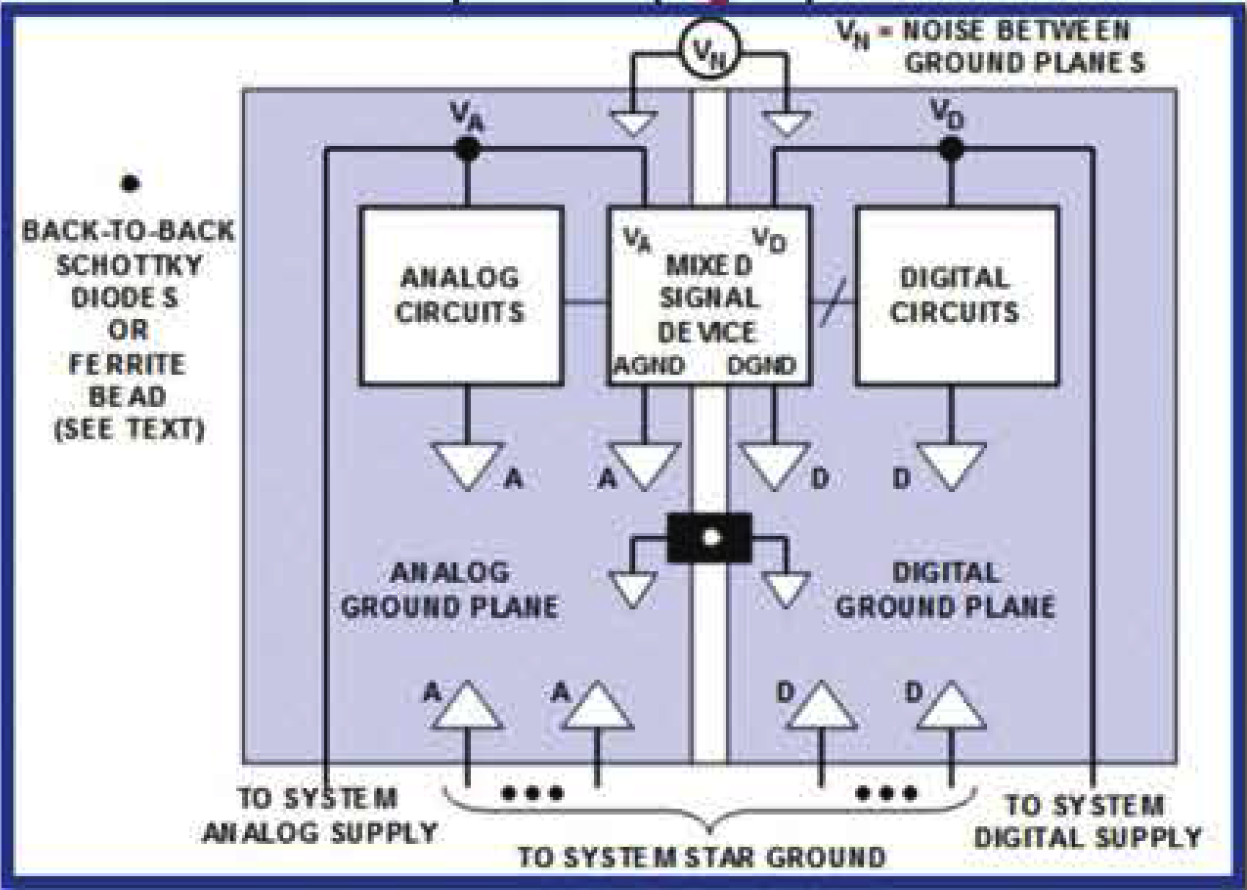
\includegraphics[width=0.35\textwidth]{images/MixedSignal4.png}\end{center}  
						 \begin{center}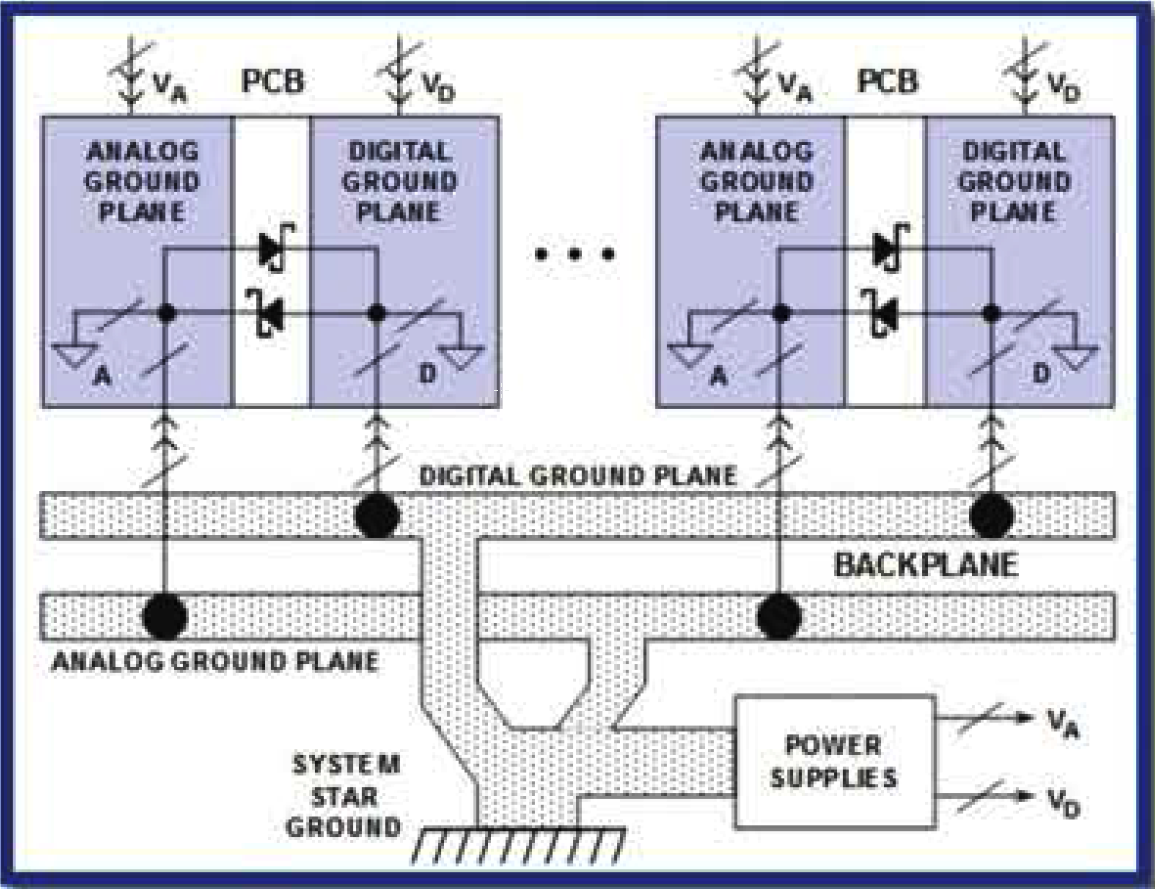
\includegraphics[width=0.35\textwidth]{images/MixedSignal5.png}\end{center}	
					\\
					\hline
					\end{tabular}
				\end{table}	
				
				
				
				\begin{table}[h!]
				\centering
				\begin{tabular}{|m{0.45\textwidth}|m{0.35\textwidth}|}

						\multicolumn{2}{c}{\textbf{Sampling Clock Circuits}}
					\\
					\hline
						\begin{itemize}
							\item Jitter on the sampling clock severely deteriorates the SNR of an ADC. 
							\item SNR of an ideal ADC (infinite resolution) exposed to a clock jitter, where $f$ is the clock frequency and $t_j$ is the sampling clock jitter is given in equation below. 
							\item Noise superposed to a clock signal translates into clock jitter. 
							\item The best solution is to create the clock locally (in the analog low noise section). 
							\item Use a low jitter oscillator such as a quartz crystal and be beware of programmable (PLL) oscillators. 
							\item If the clock comes from the digital section, try to minimize its superposed noise against AGND by transmitting it over a differential line (originating directly at the oscillator) an/or using isolation (transformer optocoupler). 
						\end{itemize}
						\begin{equation}
							SNR = 20log\left(\frac{1}{2\pi f t_j}\right)
						\end{equation}
					& 
						 \begin{center}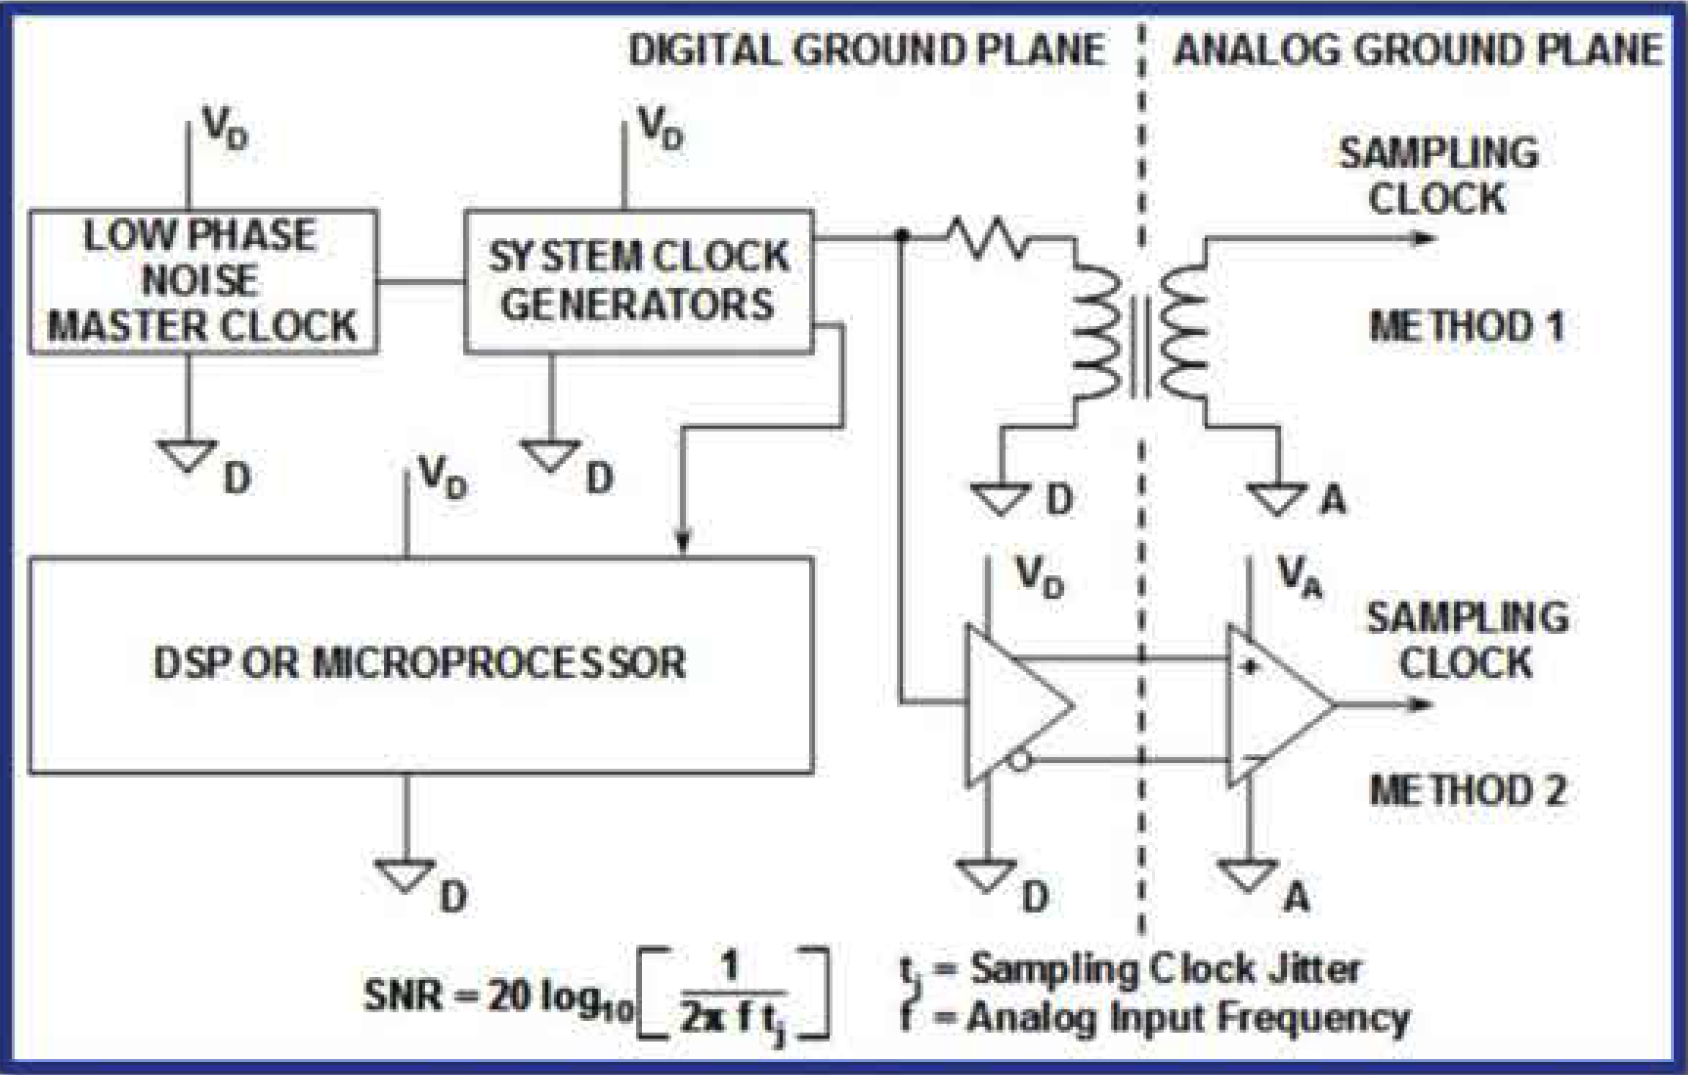
\includegraphics[width=0.35\textwidth]{images/Clock.png}\end{center}  
					\\	
					\hline
					\end{tabular}
				\end{table}	
			
				\begin{table}[h!]
				\centering
				\begin{tabular}{|m{0.45\textwidth}|m{0.35\textwidth}|}

						\multicolumn{2}{c}{\textbf{More suggestions}}
					\\
					\hline
						\begin{itemize}
							\item Split the power VCC plane: AVCC, DVCC
							\item Generally avoid splitting the GND plane! Try instead to carefully partitioning the components into analog and digital areas on the PCB. 
							\item Noisy digital return currents flow directly under the respective signal traces and do not propagate inside the analog section. 
							\item Do not route digital signal traces in the analog zone! 
							\item In case of doubt you can always design a PCB with split grounds, but provide means for connecting the two planes together at intervals of $\lambda/10$ with jumpers or zero ohm resistors. Laboratory tests will tell which solution is better. 
						\end{itemize}
					& 
						\begin{center}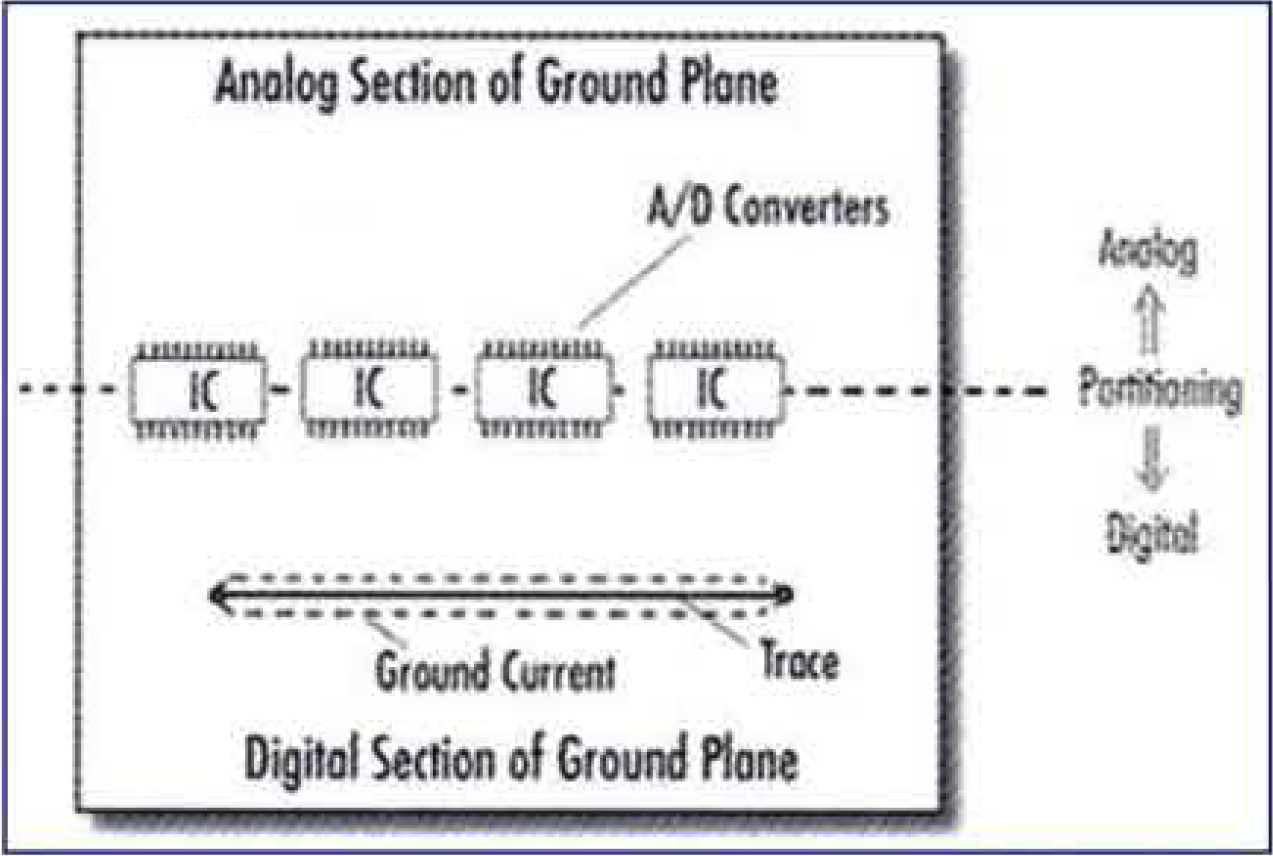
\includegraphics[width=0.35\textwidth]{images/PlaneSplit.png}\end{center}  
					\\	
					\hline
					\end{tabular}
				\end{table}	
				
				\clearpage
				\begin{table}[h!]
				\centering
				\begin{tabular}{|m{0.45\textwidth}|m{0.35\textwidth}|}
						\multicolumn{2}{c}{\textbf{How to cross a plane split with signals}}
					\\
					\hline
						\begin{itemize}
							\item Always provide a nearby path for the return signal. 
							\item It is a good place to use a common mode choke, an optocoupler or signal filters. 
							\item Another solution is to provide a bridge between the two planes (see Figure)
						\end{itemize}
					& 
						\begin{center}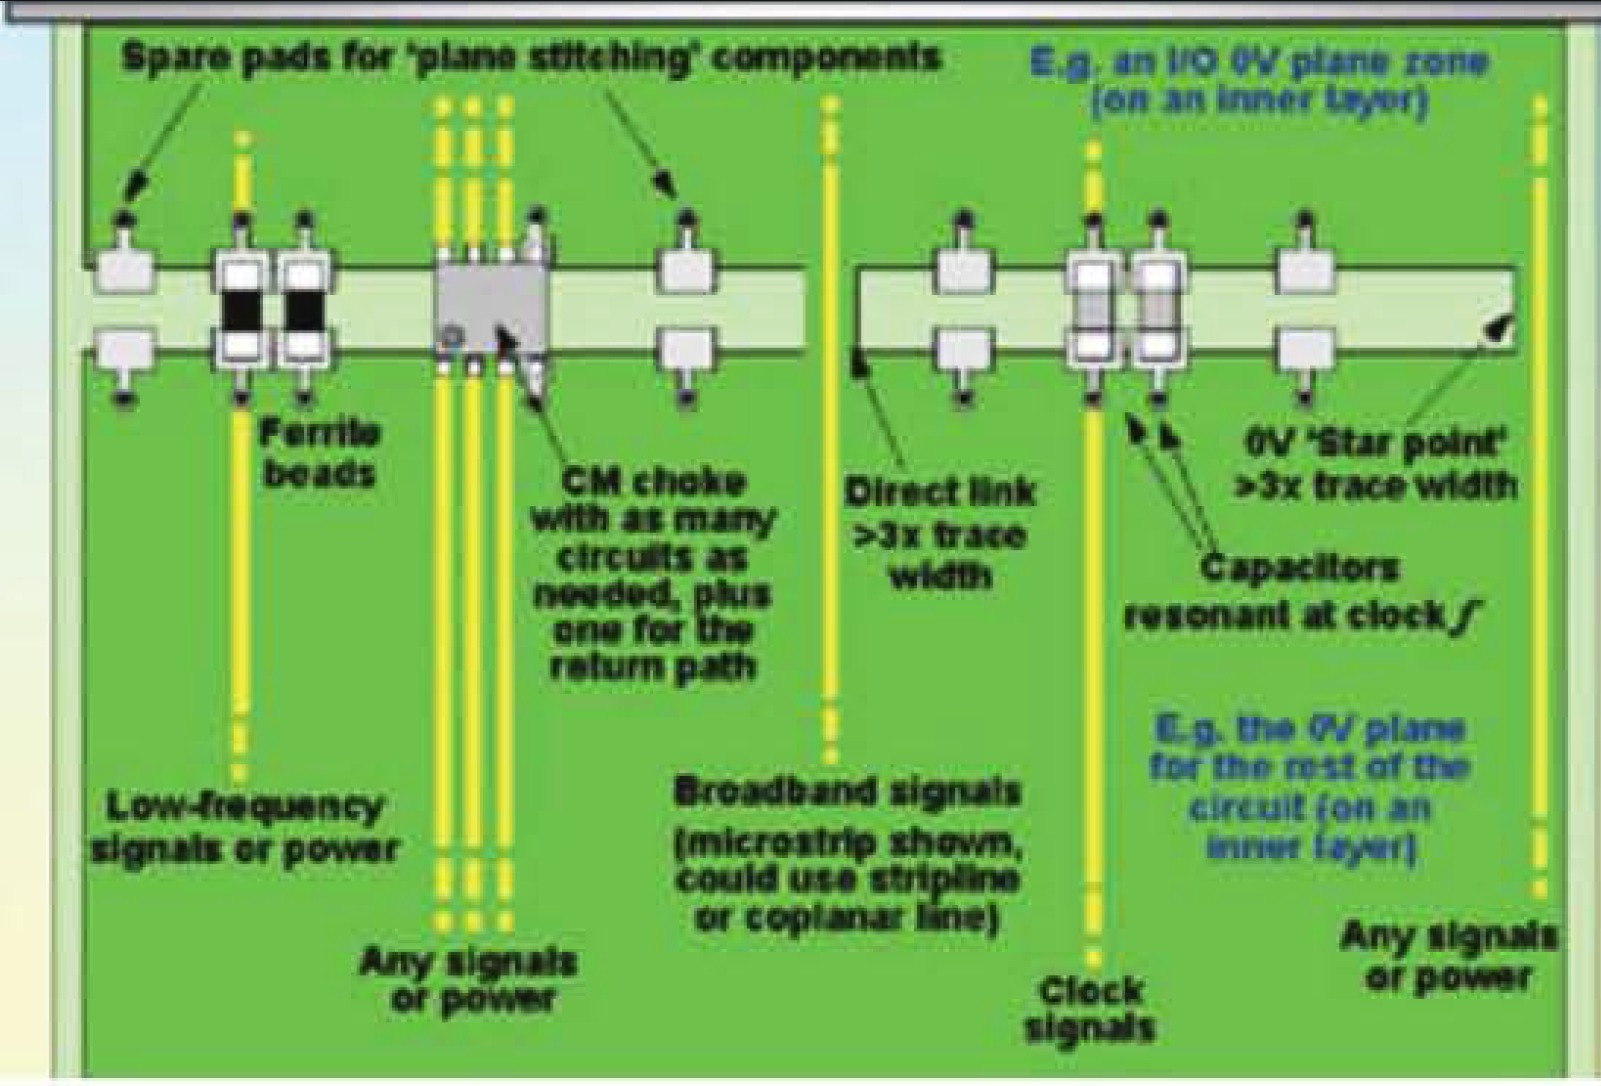
\includegraphics[width=0.35\textwidth]{images/CrossSplitPlane.png}\end{center}  
					\\	
					\hline
					\end{tabular}
				\end{table}	


			\subsubsection{Conclusions}
			\begin{itemize}
				\item Make on single reference plane!
				\item Read the recommendations of the manufacturers, purchase EvalKits and see how their PCB layout is made. 
				\item Be sceptical about AppNotes dating prior to 2003, suggesting a partitioned ground plane. Exceptions: 
				\begin{itemize}
					\item Noisy I/O sections
					\item Low frequency analog input sections with low noise or low leakage current requirements. 
				\end{itemize}
				\item It is more important to carefully partition the components and avoid placing digital signal lines inside the analog zone. 
				\item Make your PCB design so that it can be configured to various solutions (split or common GND plane, various kinds of short-lays between planes). Test will determine the most favourable layout concept. 
			\end{itemize}
			Application Example see Slides 62 to 65 from Week 2. 
			
	\subsection{Decoupling}
		It is important to reduce fluctuations on the power supply line in order to reduce emissions and guarantee correct circuit operation. The fluctuations of the power lines are due to: 
		\begin{itemize}
			\item Internal switching noise of the ICs.
			\item Vertical shoot-through of output drivers. 
			\item High charging/discharging currents of capacitive loads 
		\end{itemize}	
		$\rightarrow$ Noisy currents emit magnetic fields!\\
		$\rightarrow$ Noisy volltages emit electric fields!	
		
		\begin{table}[h!]
		\centering
		\begin{tabular}{|m{0.45\textwidth}|m{0.35\textwidth}|}
				\multicolumn{2}{c}{\textbf{Possibilities to reduce emissions from the power supply circuits:}}
			\\
			\hline
				\begin{itemize}
					\item Reduce the amplitude of the voltage fluctuations: 
					\begin{itemize}
						\item Place decoupling (bypass) capacitors between VCC and GND. 
						\item Add one for every power pin of every IC and even some more. 
					\end{itemize}
					\item Reduce current loop areas: 
					\begin{itemize}
						\item Reduce connection length between ICs and decaps. 
						\item In multilayer PCBs, place GND and VCC planes adjacent. 
						\item Take benefit from mutual inductance in the connection lines to the decap to reduce their voltage drop (impedance). This is best achieved in multilayer boards with GND and VCC planes. 
					\end{itemize}
				\end{itemize}
			& 
				\begin{center}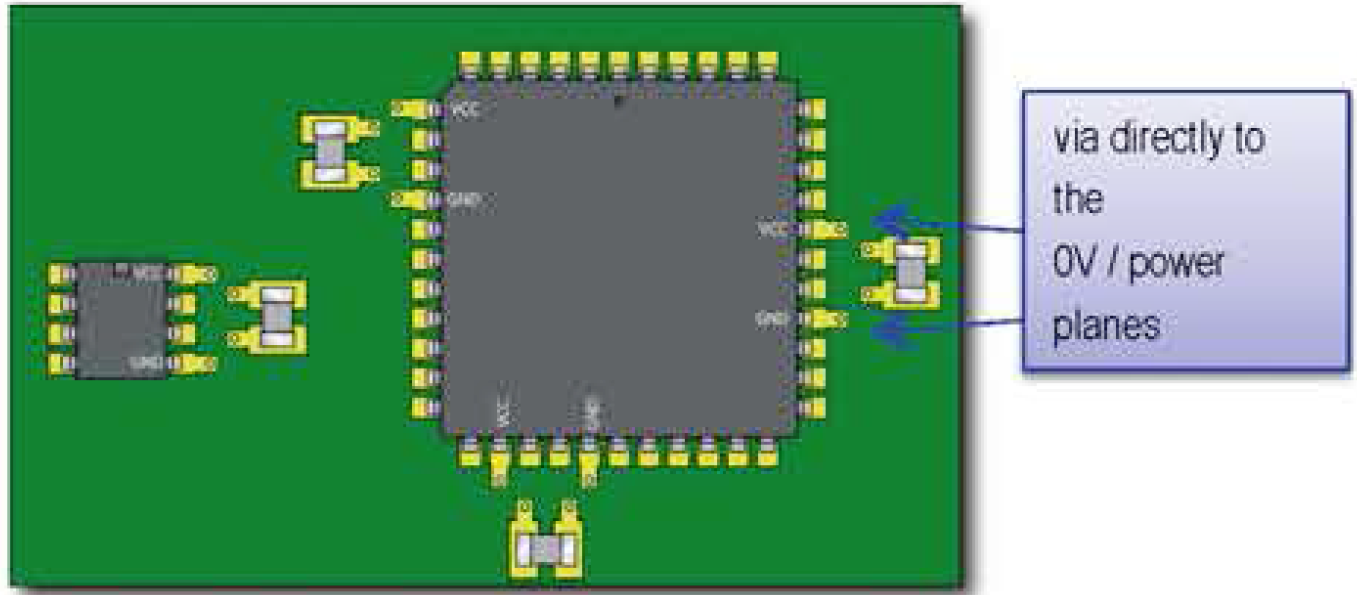
\includegraphics[width=0.35\textwidth]{images/Decaps.png}\end{center}  
				\begin{center}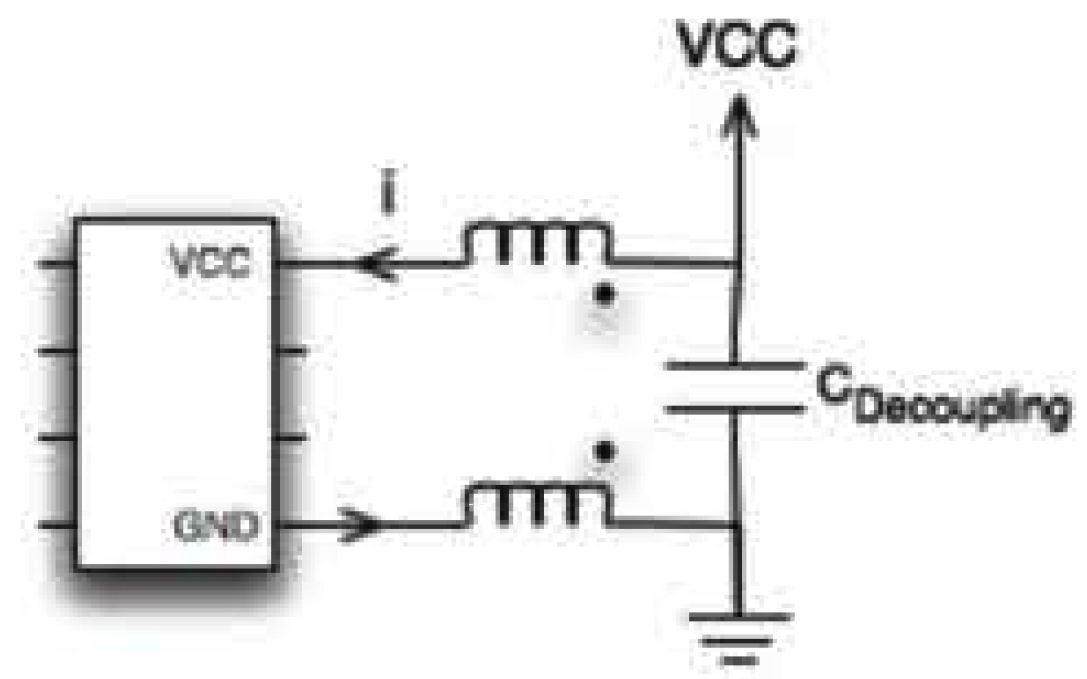
\includegraphics[width=0.35\textwidth]{images/DecapsInd.png}\end{center}  
			\\	
			\hline
			\end{tabular}
		\end{table}	


		\begin{table}[h!]
		\centering
		\begin{tabular}{|m{0.45\textwidth}|m{0.35\textwidth}|}
				\multicolumn{2}{c}{\textbf{Capacitor Series Resonance}}
			\\
			\hline
				\begin{itemize}
					\item The ESL and the C form a series resonant circuits with $\omega_{res} = \frac{1}{\sqrt{LC}}$

					\item Above the resonance frequence the capacitor behaves like an inductor!
					\item ESL depends on the capacitor case type and size, therefore: 
					\begin{itemize}
						\item Minimize PCB trace length (inductance) to decoupling capacitors as this adds to the ESL. 
						\item In multilayer PCBs, keep GND and VCC layers at a short distance to the top to reduce vias lengths. 
					\end{itemize}
					\setlength{\itemsep}{-4pt}
					\item Rule of Thumb: 
					\item[] 1 cm of thin wire (0.5 mm diameter) or 0.25 mm wide PCB trace has an L of 7 - 10 nH. 
					\item[] Therefore use smaller components with shorter leads. 
					\item[] Example: 
					\item[] 100 nF THT $\rightarrow$ $f_res$ = 8.2 MHz
					\item[] 100 nF SMD $\rightarrow$ $f_res$ = 16 MHz
				\end{itemize}
			& 
				\begin{center}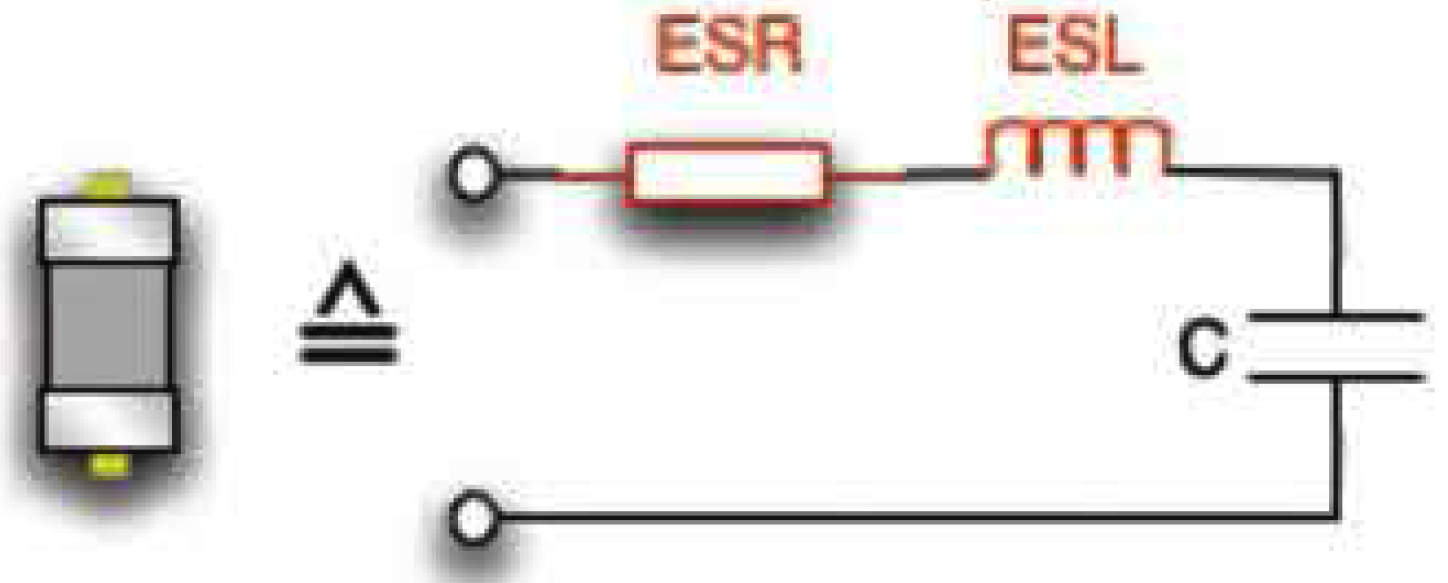
\includegraphics[width=0.35\textwidth]{images/EquivalentCircuit.png}\end{center}  
				\begin{center}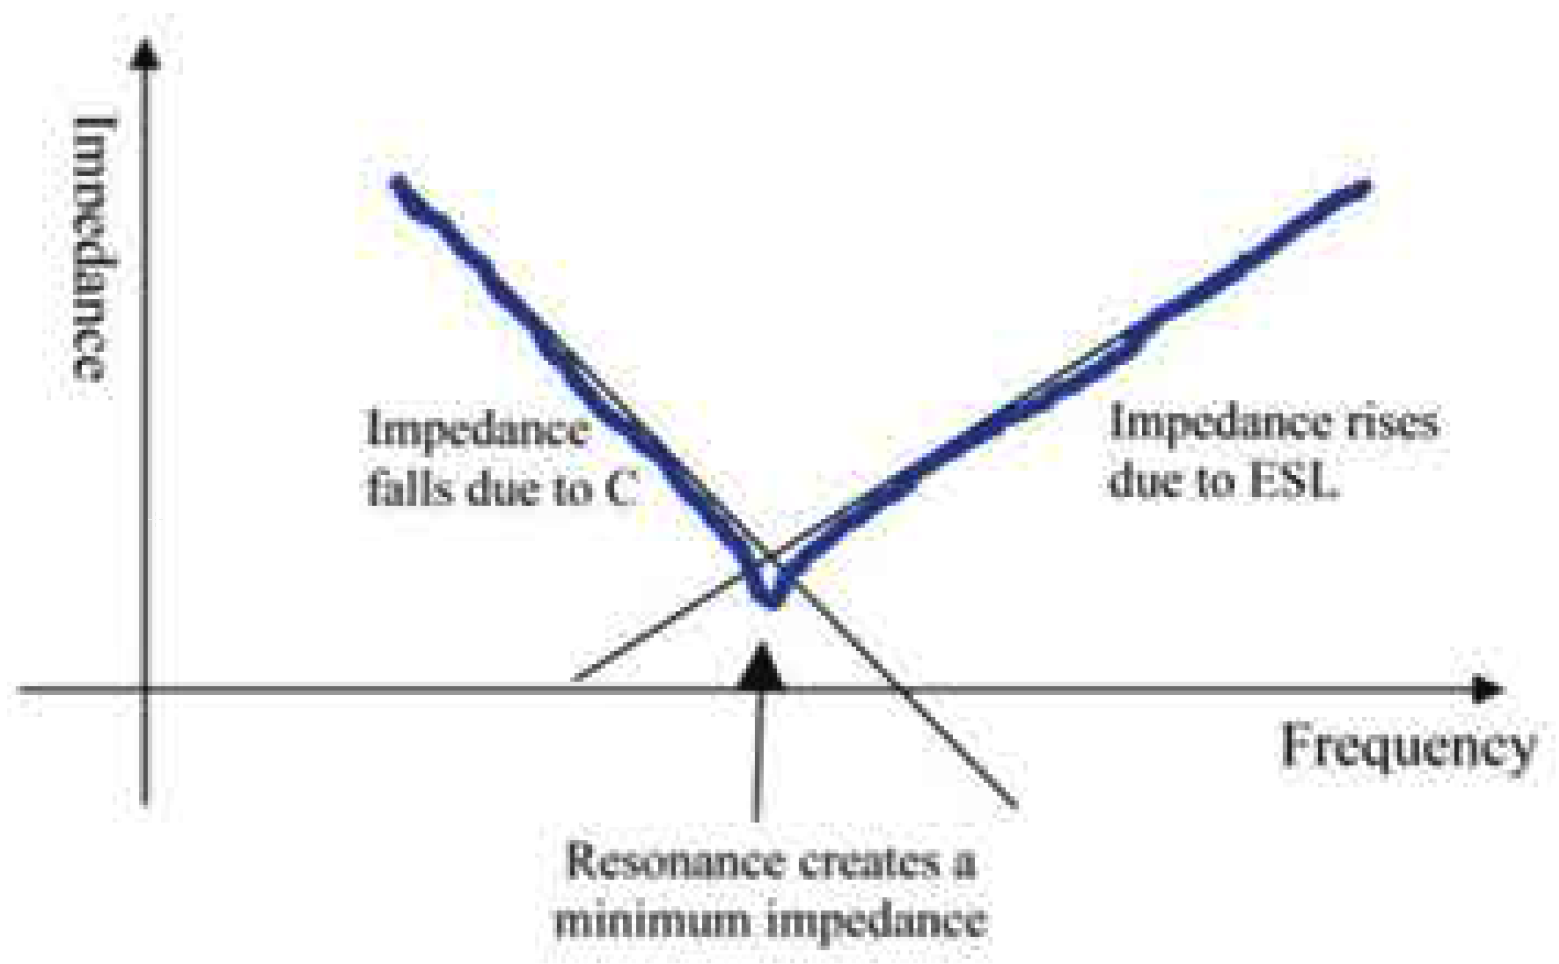
\includegraphics[width=0.35\textwidth]{images/CapImpedance.png}\end{center}  
			\\	
			\hline
			\end{tabular}
		\end{table}	
		
		\begin{table}[h!]
		\centering
		\begin{tabular}{|m{0.45\textwidth}|m{0.35\textwidth}|}
				\multicolumn{2}{c}{\textbf{Reduce external wiring}}
			\\
			\hline
				\begin{itemize}
					\item Reduce additional L due to PCB traces that add to the capacitor's ESL. 
					\item Reduce area of the loop formed by the capacitor and the IC. 
				\end{itemize}
			& 
				\begin{center}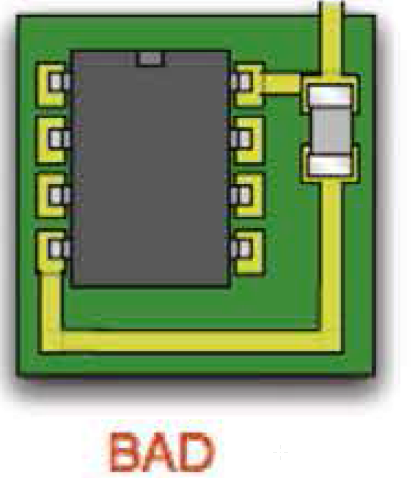
\includegraphics[width=0.15\textwidth]{images/BadTrace.png}\end{center}  
				\begin{center}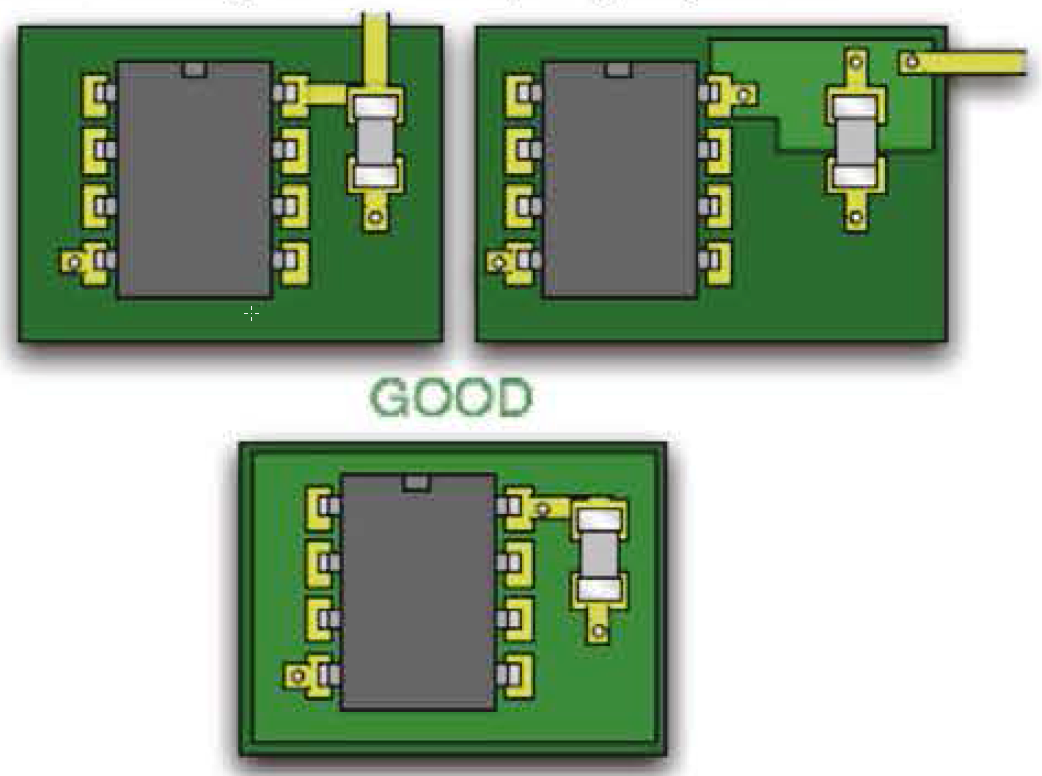
\includegraphics[width=0.25\textwidth]{images/GoodTrace.png}\end{center}  
			\\	
			\hline
			\end{tabular}
		\end{table}	
		
		\begin{table}[h!]
		\centering
		\begin{tabular}{|m{0.45\textwidth}|m{0.35\textwidth}|}
				\multicolumn{2}{c}{\textbf{Oscillator circuits}}
			\\
			\hline
				\begin{itemize}
					\item Reduce the area of the oscillator circuit
					\item Keep connections short
					\item Keep noise from GND layer out of the oscillator circuit. 
				\end{itemize}
			& 
				\begin{center}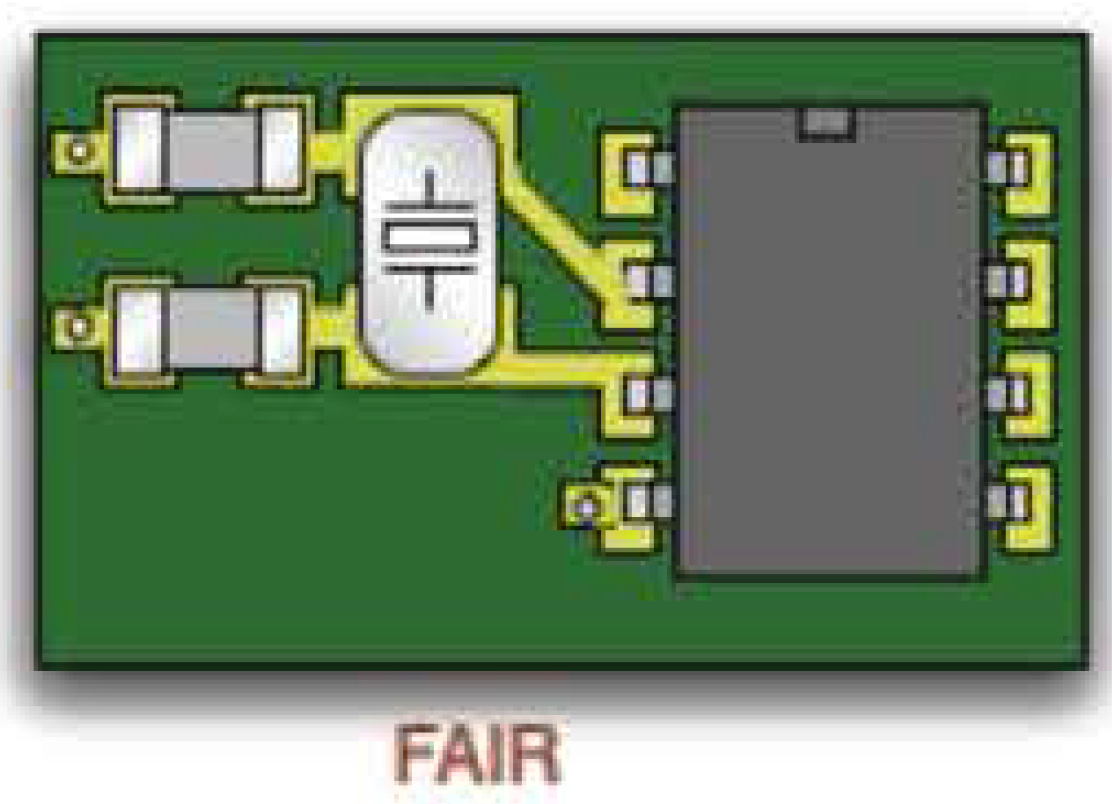
\includegraphics[width=0.25\textwidth]{images/Oszi1.png}\end{center}  
				\begin{center}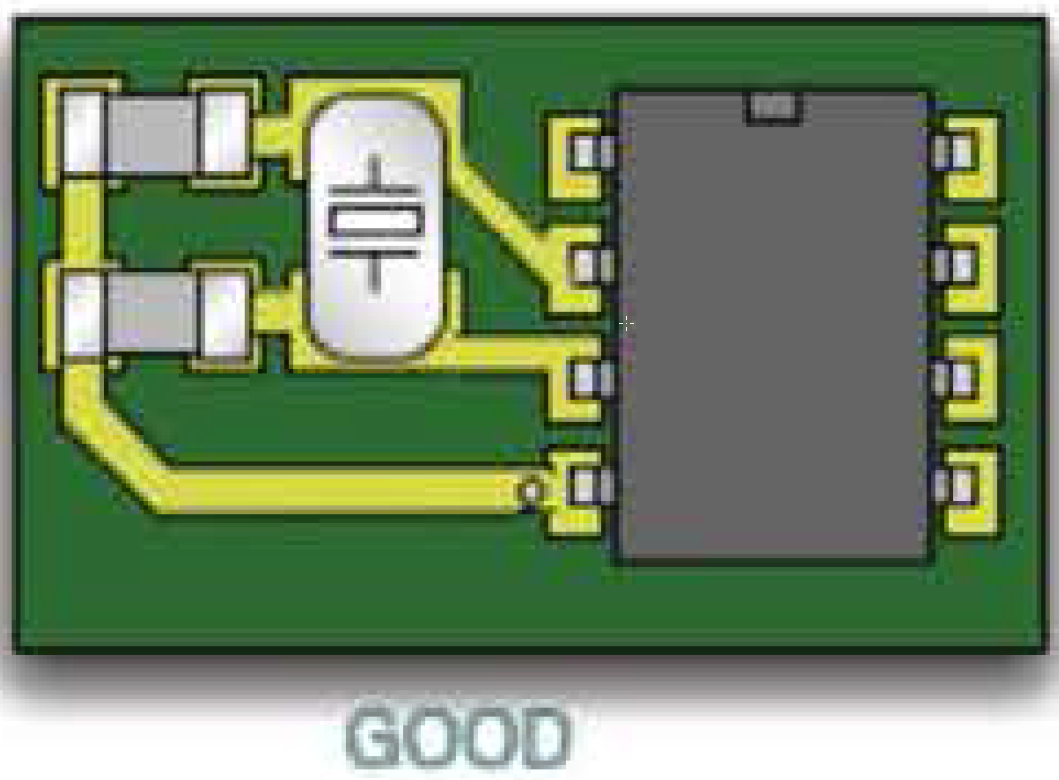
\includegraphics[width=0.25\textwidth]{images/Oszi2.png}\end{center} 
				\begin{center}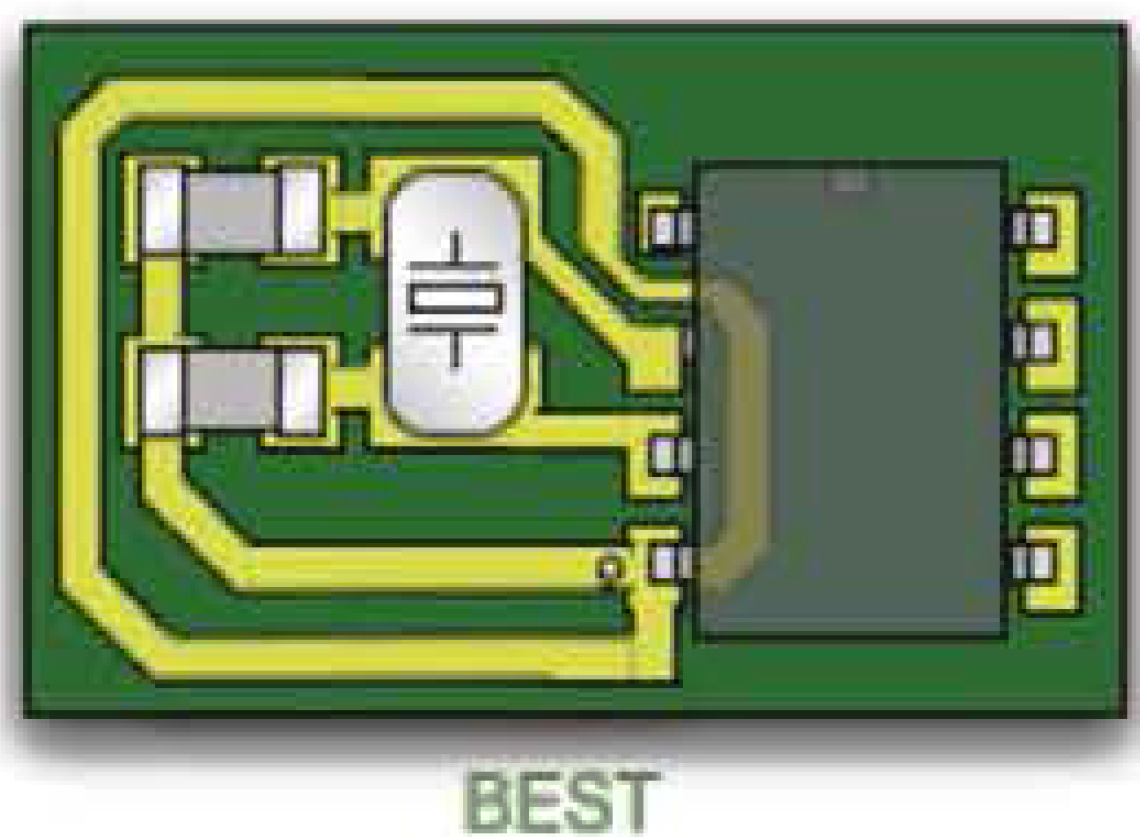
\includegraphics[width=0.25\textwidth]{images/Oszi3.png}\end{center}   
			\\	
			\hline
			\end{tabular}
		\end{table}	
		

		\begin{table}[h!]
		\centering
		\begin{tabular}{|m{0.45\textwidth}|m{0.35\textwidth}|}
				\multicolumn{2}{c}{\textbf{How to choose decoupling capacitors}}
			\\
			\hline
				\begin{itemize}
					\item Use MLCC (multilayer ceramic) capacitors: X7R $\rightarrow$ low loss, compact size
					\item Use the smallest possible SMD case $\rightarrow$ lower equivalent series inductance
					\item Commonly used values: 1nF, 10nF, 100nF
				\end{itemize}
				\begin{center}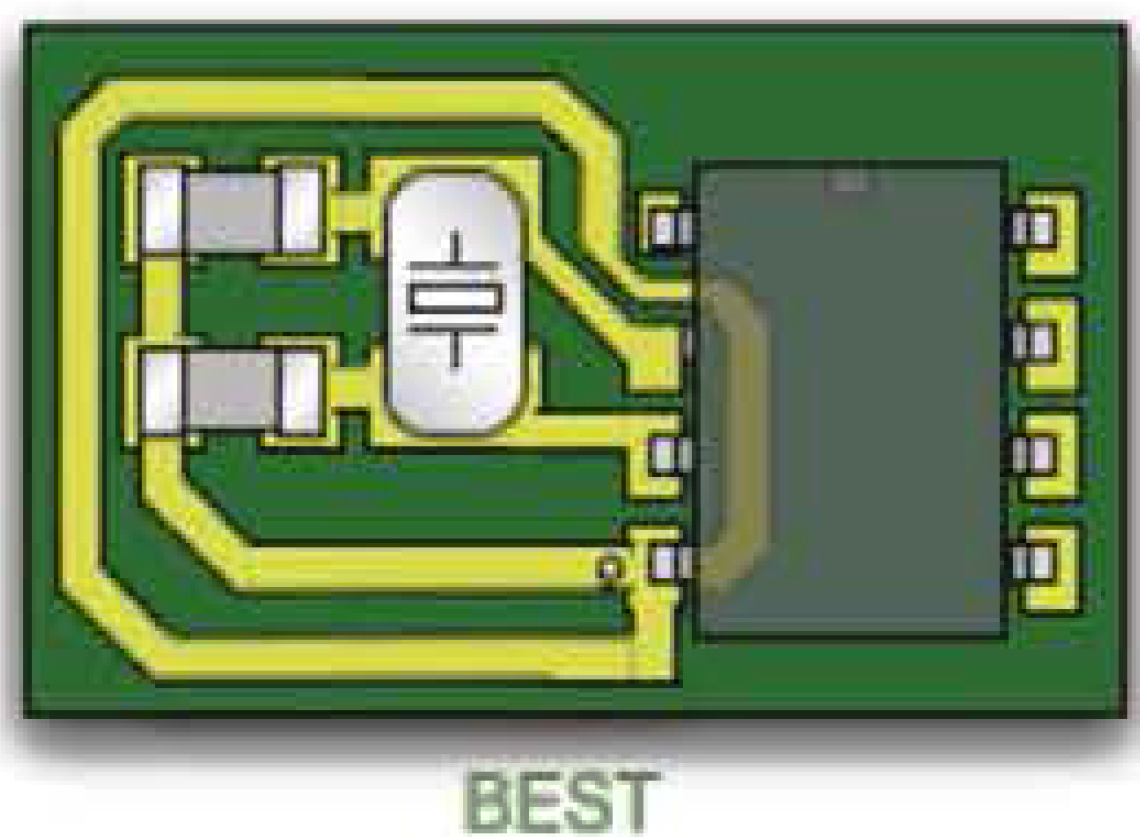
\includegraphics[width=0.2\textwidth]{images/Oszi3.png}\end{center}
			& 
				\begin{center}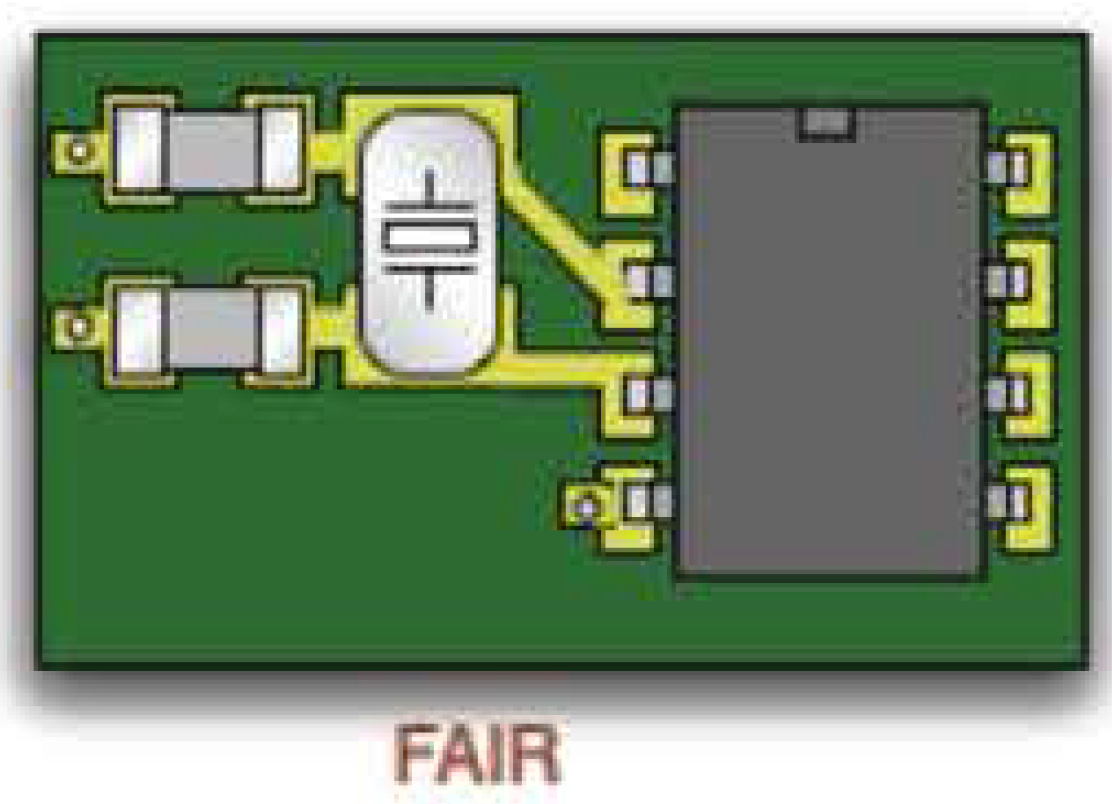
\includegraphics[width=0.2\textwidth]{images/Oszi1.png}\end{center}  
				\begin{center}\includegraphics[width=0.2\textwidth]{images/Oszi2.png}\end{center} 
				   
			\\	
			\hline
				\multicolumn{2}{c}{\textbf{Paralleling decoupling capacitors}}
			\\
			\hline
				\begin{itemize}
					\item Idea: 
					\setlength{\itemsep}{-4pt}
					\item[] Above its $\omega_{res}$ a single capacitor has an increasing Z $\rightarrow$ reduce this Z at higher frequencies with a smaller C in parallel. 
					\item The risk: 
					\setlength{\itemsep}{-4pt}
					\item[]The equivalent circuit is now of $4^{th}$ order and $Z_{TOT}(\infty)$ has 2 zeros and 3 poles. Network theory says that they alternate on the frequency axis. Therefore, between the series resonance of each single capacitor we have a frequency where Z becomes very high. 
					\setlength{\itemsep}{0pt}
					\item How to mitigate (entschärfen) parallel resonance: 
					\setlength{\itemsep}{-4pt}
					\item[] Use C with higher ESR (or add a small series R), this loss adds more damping to the parallel resonance $\rightarrow$ less Q. 
					\item[] When paralleling C's, use all C's of the same capacitance and put a great number of C's in parallel with closely spaced series resonance frequencies. 
					\setlength{\itemsep}{0pt}
					\item Still recommended in analog circuits: 
					\setlength{\itemsep}{-4pt}
					\item[] Circuits operating at frequencies below a few MHz are not affected by high frequency parallel resonances, therefore use combination of: 
					\item[] A large C (10 - 50 $\mu F$) to decouple noise introduced by the power supply
					\item[] A smaller C (100 nF) as a return path for higher frequency noise generated by the IC. 
					\setlength{\itemsep}{0pt}
					\item Placement: 
					\setlength{\itemsep}{-4pt}
					\item[] If possible take advantage of magnetic flux cancellation that reduces ESL when placing multiple capacitors very close to each other with opposite current flow. 
				\end{itemize}
			& 
					\begin{center}\includegraphics[width=0.35\textwidth]{images/ParallelC.png}\end{center}  
					\begin{center}\includegraphics[width=0.35\textwidth]{images/ParallelC2.png}\end{center} 
					\begin{center}\includegraphics[width=0.35\textwidth]{images/ParallelC3.png}\end{center} 

			\\	
			\hline
			\end{tabular}
		\end{table}	
		
		
		
		\begin{table}[h!]
		\centering
		\begin{tabular}{|m{0.45\textwidth}|m{0.35\textwidth}|}
				\multicolumn{2}{c}{\textbf{Risk of Resonance of VCC GND cavity!}}
			\\
			\hline
			
				\begin{itemize}
					\item In multilayer PCBs placing the VCC an GND planes adjacent and very close (d  $< 100\mu m$) produces a good intrinsic decoupling capacitance since $C = \varepsilon_0 \varepsilon_r \frac{A}{d}$ (FR4 with d = $100 \mu m$ $\rightarrow$ $C = 37 pF/cm^2$)
					\item Avoid the risk of resonance:
					\setlength{\itemsep}{-4pt}
					\item[] Reducing the distance between VCC and GND planes reduces their cavity's Q. 
					\item[] Resize the VCC area so that resonant frequencies along its length L and its W do not overlap $\rightarrow$ choose L/W as an irrational number! 
					\item[] Spread many decoupling caps all over the PCB, spaced smaller than $\lambda/4$ of the highest frequency of concern. 
					\item[] Partition the VCC plane into smaller planes connected through $\pi$-Filters $\rightarrow$ Shift plane resonance to higher uncritical frequencies. 
					\item[] If multiple reference planes of the same type exist, contact them with many vias, spaced at $\lambda/10$ of the highest frequency of concern. 
					\item[] Add some damping between GND and VCC (R, series R-C or capacitor with higher ESR)
					\setlength{\itemsep}{0pt}
					\item Use Ferrite beads or RF suppressors on VCC: 
					\setlength{\itemsep}{-4pt}
					\item[] Can help further suppress VCC noise from ICs, are useful when VCC is already partitioned and L or $\pi$ Filters can be implemented with ferrite beads. 
					\item[] Do not use normal inductors (resonant circuit!)
				\end{itemize}
			&
					\begin{center}\includegraphics[width=0.35\textwidth]{images/FerriteDecouple1.png}\end{center} 
					\begin{center}\includegraphics[width=0.35\textwidth]{images/FerriteDecouple2.png}\end{center} 
			\\
			\hline
			\end{tabular}
		\end{table}
	\clearpage
	\subsection{Transmission Lines}
		\begin{itemize}
			\setlength{\itemsep}{-4pt}
			\item A piece of PCB trace with a length z has a resistance of $R = \rho \frac{z}{A}$, where $A$ is the diameter area. 
			\item Current flow produces a temperature rise therefore the trace widths must be dimensioned accordingly!
			\item The capacitance formed by two copper areas on adjacent PCB layers is 37 $pF/cm^2$. 
			\item The self inductance of a PCB trace when there is no copper underneath is 
			\item[] $L = 0.00002\cdot l \left(ln\left(\frac{2l}{w+h}\right)+ 0.2235\left(\frac{w+h}{l}\right)+0.5\right) [\mu H]$, where l is the length, w the width and h the height of the copper trace. 
			\item Two parallel PCB trace have a mutual inductance M, if the mutual coupling is good (reference plane carrying the return current is very close to the signal trace) then (L-M) is very small and the voltage $\Delta V$ is very small, therefore using continuous reference planes adjacent to each signal plane is a good reason! 
			\item There is a forward $u_a$ and a reflected signal $u_b$
			\item[] $\frac{|u_a|}{|i_a|} = \frac{|u_b|}{|i_b|} = \sqrt{\frac{L'}{C'}} = Z_0$
			\item The propagation velocity within the transmission line is given by
			\item[] $v = \frac{c}{\sqrt{\varepsilon_r \mu_r}} \approx \frac{1}{\sqrt{L' C'}}$
			\item In order to avoid reflection the load impedance $Z_L$ should be equivalent to the characteristic impedance $Z_0$
			\item[] $Z_0 = Z_L$
			\item If $Z_L \neq Z_0$ there is a reflection, which is given by the reflection coefficient
			\item[] $r = \frac{u_a}{u_b}$
			\item[] $r = \frac{Z_L - Z_0}{Z_L + Z_0}$
			\item[] $Z_L = Z_0 \frac{1+r}{1-r}$
		\end{itemize}
		\begin{figure}[h]
			\centering
			\includegraphics[width=0.4\textwidth]{images/PCBTrace.png}
			\caption{Equivalent Scheme of a PCB Trace}
			\label{Fig:EqSchemePCBTrace}
		\end{figure}
		
		
		\begin{table}[h!]
		\centering
		\begin{tabular}{|m{0.45\textwidth}|m{0.35\textwidth}|}
				\multicolumn{2}{c}{\textbf{Transmission Lines on PCB}}
			\\
			\hline
				\begin{itemize}
					\item A junction between two transmission lines with different characteristic impedances generates reflections therefore be careful with width changes, connectors etc. 
					\item An unloaded ($Z_L = \infty$) trace generates reflections ($r = 1$).
					\item Splitting a trace in two ore more can generate reflections. 
					\item Sharp corners generate reflections too. 
				\end{itemize}
			&
					\begin{center}\includegraphics[width=0.35\textwidth]{images/Junction.png}\end{center} 
					\begin{center}\includegraphics[width=0.2\textwidth]{images/Stub.png}\end{center} 
					\begin{center}\includegraphics[width=0.35\textwidth]{images/ParallelTraces.png}\end{center} 
					\begin{center}\includegraphics[width=0.15\textwidth]{images/Corner.png}\end{center} 
			\\
			\hline
			\end{tabular}
		\end{table}
		
		
		\begin{table}[h!]
		\centering
		\begin{tabular}{|m{0.45\textwidth}|m{0.35\textwidth}|}
				\multicolumn{2}{c}{\textbf{Microstrip and Stripline}}
			\\
			\hline
				\begin{itemize}
					\setlength{\itemsep}{-4pt}
					\item Microstrip: 
					\item[] The signal trace runs over a continuous GND plane. 
				\end{itemize}
				\begin{equation}
					Z_0 = \frac{87}{\sqrt{\varepsilon_r + 1.41}} ln\left(\frac{5.98h}{0.8w + t}\right) \qquad [\Omega]		
				\end{equation}
				\begin{equation}
					v = \frac{1}{1.017\sqrt{0.457 \varepsilon_r + 0.67}} \qquad[ft/ns]	
				\end{equation}
				\begin{itemize}
					\setlength{\itemsep}{-4pt}
					\item Stripline: 
					\item[]The signal trace is sandwiched between two GND planes. 
				\end{itemize}
			\begin{equation}
					Z_0 = \frac{60}{\sqrt{\varepsilon_r}} ln\left(\frac{4h}{0.67\pi w \left(0.8 + \frac{t}{w}\right)}\right) \qquad[\Omega]		
				\end{equation}
				\begin{equation}
					v = \frac{1}{1.017\sqrt{\varepsilon_r}} \qquad[ft/ns]	
				\end{equation}
			&
					\begin{center}\includegraphics[width=0.35\textwidth]{images/Microstrip.png}\end{center} 
					\begin{center}\includegraphics[width=0.2\textwidth]{images/Stripline.png}\end{center} 
 
			\\
			\hline
			\end{tabular}
		\end{table}